\appendix

\section*{Supplemental material}

%===============================%
\section{Rigidity}
\label{sec:rigidity}
%===============================%



%The goal of this section is proving the Rigidity theorems used in our delegation protocols. 
We start by introducing the language required to formulate our testing results. 
%We then present a series of elementary tests, for commutation, anti-commutation,
%etc., that are presented in Sections~\ref{sec:clifford-test} and
%~\ref{sec:pauli-group}.  
%We follow by giving a test for the conjugation of one observable to another by a unitary, the Conjugation Test, in Section~\ref{sec:conj-test}.
%In Section~\ref{sec:n-clifford}, we apply the Conjugation Test  to test the
%relations that dictate how an arbitrary $m$-qubit Clifford unitary acts by
%conjugation on the Pauli matrices. In Section~\ref{sec:n-2-clifford} we
%specialize the test to the case of unitaries that can be expressed as the
%$m$-fold tensor product of Clifford observables taken from the set $\Sigma$. In
%Sections \ref{sec: RIGID test} and \ref{sec: TOM test}, we decribe variants of
%the test from Section \ref{sec:n-2-clifford}, which are later employed in the
%Leash and Dog-Walker protocols.


%============================%
\subsection{Testing}
\label{sec:general-rigidity}
%============================%

In this section we recall the standard formalisms from self-testing, including state-dependent distance measure, local isometries, etc. We also introduce a framework of ``tests for relations'' that will be convenient to formulate our results. 


\subsubsection{Distance measures}

Ultimately our goal is to test that a player implements a certain tensor product of single-qubit or two-qubit measurements defined by observables such as $\sigma_X$, $\sigma_Y$, or $\sigma_G$. Since it is impossible to detect whether a player applies a certain operation $X$ on state $\ket{\psi}$, or $VXV^\dagger$ on state $V\ket{\psi}$, for any isometry $V:\Lin(\mH)\to\Lin(\mH')$ such that $V^\dagger V = \Id$, we will (as is standard in testing) focus on testing identity up to \emph{local isometries}. Towards this, we introduce the following important piece of notation: 

\begin{definition}
For finite-dimensional Hilbert spaces $\mH_{\reg{A}}$ and $\mH_{\reg{A}'}$, $\delta>0$, and operators $R \in\Lin(\mH_{\reg{A}})$ and $S\in\Lin(\mH_{\reg{A}'})$ we say that $R$ and $S$ are $\delta$-isometric with respect to $\ket{\psi} \in \mH_{\reg{A}} \otimes \mH_{\reg{B}}$, and write $R\simeq_\delta S$, if there exists an isometry $V:\mH_{\reg{A}}\to\mH_{\reg{A}'}$ such that 
$$\big\|( R-V^\dagger SV)\otimes \Id_{\reg{B}} \ket{\psi}\big\|^2=O(\delta).$$
When $R = \{R_a\}$ and $S=\{S_a\}$ are POVM with the same set of outcomes we write $R_a \simeq_\delta S_a$ to mean
$$\sum_a \big\|( R_a-V^\dagger S_a V)\otimes \Id_{\reg{B}} \ket{\psi}\big\|^2=O(\delta).$$
If $V$ is the identity, then we further say that $R$ and $S$ are $\delta$-equivalent, and write $R\approx_\delta S$ for $\| ( R- S) \otimes \Id_{\reg{B}} \ket{\psi}\|^2=O(\delta)$.
\end{definition}

The notation $R\simeq_\delta S$ carries some ambiguity, as it does not specify the state $\ket{\psi}$. The latter should always be clear from context: we will often simply write that $R$ and $S$ are $\delta$-isometric, without explicitly specifying $\ket{\psi}$ or the isometry. The relation is transitive, but not reflexive: the operator on the right will always act on a space of dimension at least as large as that on which the operator on the left acts. The notion of $\delta$-equivalence is both transitive (its square root obeys the triangle inequality) and reflexive, and we will use it as our main notion of distance. 

\subsubsection{Strategies}

Given a two-player game, or test, a strategy for the players consists of a bipartite entangled state $\ket{\psi} \in \mH_\reg{A} \otimes \mH_\reg{B}$ together with families of projective  measurements $\{W^a_\reg{A}\}$ for Alice and $\{W_\reg{B}^a\}$ for Bob, one for each question $W$ that can be sent to either player in the test. (We often use the same symbol, a capital letter $X,Z,W,\ldots,$ to denote a question in the game and the associated projective measurement $\{W^a\}$ applied by the player upon reception of that question.) 
 Recall that to a projective measurement with outcomes in $\{0,1\}^n$ we  associate a family of observables $W(u)$ parametrized by $n$-bit strings $u\in\{0,1\}^n$, defined by $W(u) = \sum_a (-1)^{u\cdot a} W^a$. If $n=1$ we simply write $W=W(1)=W^0-W^1$; note that $W(0)=\Id$.

As already mentioned, for convenience we restrict our attention to pure-state strategies employing projective measurements. 
We will loosely refer to a strategy for the players as $(W,\ket{\psi})$, with the symbol $W$ referring to the complete set of projective measurements used by the players in the game.

\subsubsection{Consistency tests}
\label{sec:cons-test}

We formulate our tests as two-player games in which both players are treated symmetrically. Specifically, when in a test we write ``send one player the question $X$ and the other the question $Y$'' we implicitly mean that the role of ``first player'' and ``second player'' have been assigned at random, and moreover a player only gets told its question, not its ``role'' as assigned by the referee. 
 Taking advantage of this symmetry we often omit the subscript $\reg{A}$ or $\reg{B}$, as all statements involving observables for one player hold verbatim with the other player's observables as well. 

With the exception of the Tomography Test $\tom$ presented in Section~\ref{subsec:tomography}, 
all the games tests we consider implicitly include a ``consistency test'' which is meant to enforce that whenever both players are sent identical questions, they produce matching answers.\footnote{Here by a ``test'' we mean a named test, such as $\conj(A,B,R)$ or $\act(X,Z)$. Since $\conj(A,B,R)$ uses $\act(X,Z)$ as a subroutine, both the named subtest $\act(X,Z)$ and the named test $\conj(A,B,R)$ are endowed with an additional consistency test.} More precisely, let $T$ be any of the two-player tests described in the paper. Let $\Pr_T(W,W')$ be the distribution on questions $(W,W')$ to the players that is specified by $T$. Since the players are always treated symmetrically, $\Pr_T(\cdot,\cdot)$ is permutation-invariant. Let $\Pr_T(\cdot)$ denote the marginal on either player. Then, instead of executing the test $T$ as described, the verifier performs the following: 
\begin{enumerate}
\item[(i)] With probability $1/2$, execute $T$.
\item[(ii)] With probability $1/2$, select a random question $W$ according to $\Pr_T(W)$. Send $W$ to both players. Accept if and only if the players' answers are equal. 
\end{enumerate}
Then, success with probability at least $1-\eps$ in the modified test implies success with probability at least $1-2\eps$ in the original test, as well as in the consistency test. If $\{W_{\reg{A}}^a\}$ and $\{W_{\reg{B}}^b\}$ are the players' corresponding projective measurements and $\ket{\psi}_{\reg{AB}}$ their shared state, the latter condition implies 
\begin{align}
\sum_a \|(W_{\reg{A}}^a \otimes \Id - \Id \otimes W_{\reg{B}}^a)\ket{\psi}_{\reg{AB}}\|^2 &= 2-2 \sum_a \bra{\psi}_{\reg{AB}} W_{\reg{A}}^a \otimes W_{\reg{B}}^a \ket{\psi}_{\reg{AB}} \notag\\ 
&\leq 4 \eps,\label{eq:consistency}
\end{align}
so that $W_{\reg{A}}^a \otimes \Id \approx_{\eps} \Id \otimes
W_{\reg{B}}^a$ (where the condition should be interpreted on average over the
choice of a question $W$ distributed as in the test). Similarly, if
$W_{\reg{A}}$, $W_{\reg{B}}$ are observables for the players that succeed in the
consistency test with probability $1-2\eps$ we obtain $W_{\reg{A}}\otimes \Id
\approx_{\eps} \Id \otimes W_{\reg{B}}$. We will often use both relations to ``switch'' operators from one player's space to the other's; as a result we will also often omit an explicit specification of which player's space an observable is applied to. 


\subsubsection{Relations}

We use $\mathcal{R}$ to denote a set of relations over matrix variables $X,Z,W,\ldots,$ such as
$$\mathcal{R}=\big\{XZXZ=-\Id,\, HX=ZH,\,X,Z,H\in\Obs\big\}.$$
Here the constraint $X\in\Obs$ is itself a pair of relations, $X=X^\dagger$ and $X^2=\Id$ (since we consider only binary observables). Each relation implicitly imposes that the variables that appear in it have compatible dimension, e.g.\ $XZXZ=-\Id$ imposes that $X,Z$ have the same dimension. 
We only consider relations that can be expressed in the form of  one of the following
equations:
\begin{itemize}
  \item  $(-1)^a W_1\cdots W_k = \Id$, where the $W_i$ are (not necessarily distinct) unitary variables and $a\in\Z_2$, or
  \item $ W_1 \cdot ( \sum_a \omega_a W_2^a)=\Id$, where $W_1$ is a unitary variable, $\{W_2^a\}$ a projective measurement with $s$ possible outcomes, and $\omega_a$ are (arbitrary) $s$-th roots of unity.
\end{itemize}
Here what we mean by ``unitary variable'' (resp. ``projective measurement'') is that when saying that a collection of matrices satisfy the relation, we always require that the matrices are unitary (resp. a projective measurement); if they are not then by definition they do not satisfy the relation. 

\begin{definition}[Rigid self-test]
We say that a set of relations $\mathcal{R}$ is $(c,\delta(\eps))$-testable, on average under the distribution $\mathcal{D}:\mathcal{R}\to[0,1]$, if
  there exists a game (or test) $G$ with question set $\mathcal{Q}$ such that the following holds. The set $\mathcal{Q}$ includes (at least) a symbol for each variable in $\mathcal{R}$ that is either
  an observable or a POVM. Moreover,
\begin{itemize}
\item (\emph{Completeness}) There exists a set of operators which exactly satisfy all relations in $\mathcal{R}$ and a strategy for the players which uses these operators for the questions in $\mathcal{Q}$ that correspond to symbols appearing in the relations $\mathcal{R}$ (together possibly with others for the additional questions) that has success probability at least $c$;
\item (\emph{Soundness}) For any $\eps>0$ and any strategy $(W,\ket{\psi}_{AB})$ that succeeds in the game with probability at least $c-\eps$, the associated measurement operators satisfy the relations in $\mathcal{R}$ up to $\delta(\eps)$. More precisely, on average
 over the choice of a relation $f(W)=\Id$ from $\mathcal{R}$ chosen according to $\mathcal{D}$, it holds that $\|  (f(W)-\Id)\otimes\Id \ket{\psi}_{\reg{AB}}\|^2 \leq \delta(\eps)$.
\end{itemize}
If both conditions hold, we also say that the game $G$ is a robust $(c,\delta(\eps))$ self-test for the relations $\mathcal{R}$. 
\end{definition}

Most of the games we consider have perfect completeness, $c=1$, in which case we  omit explicitly mentioning the parameter. 
 The distribution $\mathcal{D}$ will often be implicit from context, and we do not always specify it explicitly (e.g. in case we only measure $\delta(\eps)$ up to multiplicative factors of order $|\mathcal{R}|$ the exact distribution $\mathcal{D}$ does not matter as long as it has complete support). 

\begin{definition}[Stable relations]
We say that a set of relations $\mathcal{R}$ is $\delta(\eps)$-stable, on average under the distribution $\mathcal{D}:\mathcal{R}\to[0,1]$, if for any state $\ket{\psi}\in\mH_\reg{A}\otimes \mH_\reg{B}$ and families of operators $W_A\in\Lin(\mH_\reg{A})$ and  $W_B\in\Lin(\mH_\reg{B})$ that are consistent on average, i.e. 
$$\Es{f \sim\mathcal{D}} \Es{W \in_U f} \big\| (\Id\otimes W_B - W_A \otimes \Id)\ket{\psi}\big\|^2\leq \eps,$$
where $W \in_U f$ is shorthand for $W$ being a uniformly random operator among those appearing in the relation specified by $f$,
and satisfy the relations on average, i.e. 
$$\Es{\substack{f\sim\mathcal{D}:\\f(W)=\Id \in\mathcal{R}}} \big\|  (f(W_A)- \Id) \otimes \Id \ket{\psi}\big\|^2 \leq \eps,$$
  there exists operators $\hat{W}$ which satisfy the same relations exactly and are $\delta(\eps)$-isometric to the $W$ with respect to $\ket{\psi}$, on average over the choice of a random relation in $\mathcal{R}$ and a uniformly random $W$ appearing in the relation, i.e. there exists an isometry $V_A$ such that 
  \begin{equation}
    \Es{f \sim\mathcal{D}} \Es{W \in_U f} \big\|( \hat{W}_A-V_A W_A)\otimes \Id \ket{\psi}\big\|^2=O(\delta(\eps)).\nonumber
  \end{equation}
	\end{definition}


%---------------------------%
\subsection{The conjugation test}
\label{sec:conj-test}
%---------------------------%

We give a test which certifies that a unitary (not necessarily an observable) conjugates one observable to another. More precisely, let $A,B$ be observables and $R$ a unitary acting on the same space $\mH$. The test $\conj(A,B,R)$ certifies that the players implement observables of the form
\begin{equation}\label{eq:def-xr}
X_R = \begin{pmatrix} 0 & R^\dagger\\ R & 0 \end{pmatrix}\qquad \text{and}\qquad C = C_{A,B} = \begin{pmatrix} A & 0\\ 0 & B \end{pmatrix}
\end{equation}
such that $X_R$ and $C$ commute. The fact that $X_R$ is an observable implies that $R$ is unitary,\footnote{Note that $R$ will not be directly accessed in the test, since by itself it does not necessarily correspond to a measurement.} while the commutation condition is equivalent to the relation $RAR^\dagger = B$. The test thus tests for the relations
\begin{align*}
 \mathcal{C}\{R,C\} &= \big\{ X_R,C,X,Z\in \Obs\big\} \cup \big\{XZ=-ZX\big\}
\cup \big\{ X_R C = C X_R,\, X_RZ=-Z X_R,\, C Z=ZC\big\}.
\end{align*}
Here the anti-commuting observables $X$ and $Z$ are used to specify a basis in which $X_R$ and $C$ can be block-diagonalized. The anti-commutation and commutation relations with $Z$ enforce that $X_R$ and $C$ have the form described in~\eqref{eq:def-xr}.
These relations are enforced using commutation and anti-commutation tests that are standard in the literature on self-testing. For convenience, we state those tests, $\comt$ and $\act$, in Appendix~\ref{sec:clifford-test}. The conjugation test, which uses them as sub-tests, is given in Figure~\ref{fig:conjugation-test-1}. Here, ``Inputs'' refers to a subset of designated questions in the test; ``Relation'' indicates a relation that the test aims to certify; ``Test'' describes the certification protocol. (Recall that all our protocols implicitly include a ``consistency test, not specified on the figure, in which a question is chosen uniformly at random from the marginal distribution and sent to both players, whose answers are accepted if and only if they are equal.)

\begin{figure}[H]
\rule[1ex]{\textwidth}{0.5pt}\\
Test~\conj(A,B,R) 
\begin{itemize}
    \item Inputs: $A$, $B$, $X$, $Z$, $X_R$ and $C$ observables.
    \item Relations:  $\mathcal{C}\{R,C\} $, with $R$ defined from $X_R$, and $C$ related to $A$ and $B$, as in~\eqref{eq:def-xr}. 
    \item Test: execute each of the following with equal probability
		\begin{enumerate}
\item[(a)] With probability $1/8$ each, execute tests $\act(X,Z)$,  $\comt(C,Z)$, $\comt(X_R,C)$,   $\act(X_R,Z)$ and $\comt(A,X)$, $\comt(B,X)$, $\comt(A,Z)$, $\comt(B,Z)$. 
\item[(b)] Ask one player to measure $A$, $B$, $C$ or $Z$ (with probability $1/4$ each), and the other to jointly measure $A$ or $B$ (with probability $1/2$ each) and $Z$. The first player returns one bit, and the second two bits. Make an acceptance decision as follows: 
\begin{itemize}
\item If the first player was asked $C$ and the second player was asked $(A,Z)$ then accept \emph{unless} the second player's second answer bit is~$0$ and his first answer bit does not match the first player's;
\item If the first player was asked $C$ and the second player was asked $(B,Z)$ then accept \emph{unless} the second player's second answer bit is~$1$ and his first answer bit does not match the first player's;
\item If the first player was asked $A$, $B$, or $Z$ then accept if and only if his answer bit matches the corresponding answer from the second player.
\end{itemize}
In all other cases, accept. 
\end{enumerate}
\end{itemize}
\rule[2ex]{\textwidth}{0.5pt}\vspace{-0.5cm}
\caption{The conjugation test, $\conj(A,B,R)$.}
\label{fig:conjugation-test-1}
\end{figure}

\begin{lemma}\label{lem:conj}
The test $\conj(A,B,R)$ is a $(1,\delta)$ self-test for the set of relations
  $\mathcal{C}\{R,C\}$, for some $\delta = O(\sqrt{\eps})$. Moreover, for any
  strategy that succeeds with probability at least $1-\eps$ in the test it holds
  that $C \approx_{\delta} A  (\Id+Z)/2 + B
 (\Id-Z)/2$, where $A,B,C$ and $Z$ are the observables applied by the prover on receipt of a question with the same label. 
\end{lemma}

\begin{proof}
Completeness is clear, as players making measurements on a maximally entangled state on $\mH_{\reg{A}}\otimes \mH_{\reg{B}}$, tensored with an EPR pair on $\C^2_{\reg{A}'} \otimes \C^2_{\reg{B}'}$ for the $X$ and $Z$ observables, and using $X_R$ and $C$ defined in~\eqref{eq:def-xr} (with the blocks specified by the space associated with each player's half-EPR pair) succeed in each test with probability $1$. 

We now consider soundness. Success in $\act(X,Z)$ in part (a) of the test implies the existence of local isometries $V_A,V_B$ such that $V_A:\mH_\reg{A}\to \mH_{\hat{\reg{A}}}\otimes \C^2_{\reg{A}'}$, with $X\simeq_{\sqrt{\eps}} \Id_{\hat{\reg{A}}}\otimes \sigma_X$ and $Z\simeq_{\sqrt{\eps}} \Id_{\hat{\reg{A}}}\otimes\sigma_Z$. By Lemma~\ref{lem:pauli-c}, approximate commutation with both $X$ and $Z$ enforced by the tests $\comt(A,X)$, $\comt(A,Z)$, $\comt(B,X)$ and $\comt(B,Z)$ implies that under the same isometry, 
\begin{equation}\label{eq:cliff-2c}
A\simeq_{\sqrt{\eps}} A_I \otimes \Id\qquad\text{and}\qquad B\simeq_{\sqrt{\eps}} B_I \otimes \Id\;,
\end{equation}
 for observables $A_I, B_I$ on $\mH_{\hat{\reg{A}}}$. Similarly, the parts of the test involving $C$ and $X_R$ imply that they each have the block decomposition specified in~\eqref{eq:def-xr}. 
In particular, using the second part of Lemma~\ref{lem:pauli-c-n} (with $n=1$ and $c=1$, exchanging the roles of $Z$ and $X$) it follows that anti-commutation of $X_R$ with $Z$ certifies that $X_R$ has  a decomposition of the form  
\begin{equation}\label{eq:xr-1}
X_R \simeq_{\sqrt{\eps}} R_X \otimes \sigma_X + R_Y \otimes \sigma_Y\;.
\end{equation}
Let $R = ( R_X + i R_Y)| R_X + i R_Y|^{-1}$, so that $R$ is unitary. Note that since $X_R$ is an observable, $X_R^2=\Id$, and so it follows from~\eqref{eq:xr-1} that $(R_X+iR_Y)(R_X+iR_Y)^\dagger \otimes \Id \simeq_{\sqrt{\eps}} \Id$. Thus $R \simeq_{\sqrt{\eps}} R_X + i R_Y$. 
 Similarly, using the first part of Lemma~\ref{lem:pauli-c-n} commutation of $C$ with $Z$ implies that 
\begin{equation}\label{clif-2ab}
C \simeq_{\sqrt{\eps}} C_I \otimes \sigma_I + C_Z \otimes \sigma_Z\;,
\end{equation}
 for Hermitian $C_I$, $C_Z$ such that $C_I \pm C_Z$ are observables because $C$ is an observable. 

Next we analyze part (b) of the test. Let $\{W_{AZ}^{a,z}\}$ be the projective measurement applied by the second player upon query $(A,Z)$. Success with probability $1-O(\eps)$ conditioned on the questions being $C$ and $(A,Z)$ item ensures that 
\begin{equation}\label{clif-2b}
\big| \bra{\psi} C^0 \otimes (W_{AZ}^{00} + W_{AZ}^{01} + W_{AZ}^{11}) + C^1\otimes (W_{AZ}^{10} + W_{AZ}^{01} + W_{AZ}^{11}) \ket{\psi} \big| \,\geq\,1-O(\eps),
\end{equation}
and a similar condition holds for the case $C$ and $(B,Z)$, with $W_{BZ}$ instead of $W_{AZ}$. 

Success with probability $1-O(\eps)$ in the case of questions $A$, $B$ or $Z$ and $(A,Z)$ or $(B,Z)$ respectively ensures consistency of $\{W_{AZ}^{a,z}\}$ (resp.\ $\{W_{BZ}^{b,z}\}$) with the observable $A$ (resp.\ $B$) when marginalizing over the second outcome, and $Z$ when marginalizing over the first outcome. Since $A$ (resp. $B$) and $Z$ approximately commute, using the decompositions for $A$ and $B$ derived in~\eqref{eq:cliff-2c} it follows that $W_{AZ} \simeq_{\sqrt{\eps}} A_I \otimes \sigma_Z$ and $W_{BZ} \simeq_{\sqrt{\eps}} B_I \otimes \sigma_Z$. 

Similarly regarding the observable $C$, using that we already showed in~\eqref{clif-2ab} that $C$ is block-diagonal in the basis specified by $X$ and $Z$,~\eqref{clif-2b} and $W_{AZ} \simeq_{\sqrt{\eps}} A_I \otimes \sigma_Z$ gives $(C_I^0 + C_Z^0) \simeq_{\sqrt{\eps}} A_I^0$ and $(C_I^1 + C_Z^1) \simeq_{\sqrt{\eps}} A_I^1$. Using the analogous relations for $W_{BZ}$ we get $(C_I - C_Z) \simeq_{\sqrt{\eps}} B_I$. Thus $C_I \simeq_{\sqrt{\eps}} (A+B)/2$ and $C_Z \simeq_{\sqrt{\eps}} (A-B)/2$. This shows the ``Moreover'' part of the lemma. 

Finally, success in test $\comt(X_R,C)$ certifies the approximate commutation relation $[X_R,C]\simeq_{\sqrt{\eps}} 0$, which, given the decomposition of $X_R$ and $C$ obtained so far, implies $RA \simeq_{\sqrt{\eps}} B R$, as desired. 
\end{proof}



\subsection{Testing Clifford unitaries}
\label{sec:n-clifford}

Let $m\geq 1$ be an integer, and $R$ an $m$-qubit Clifford unitary. $R$ is characterized, up to phase, by its action by conjugation on the $m$-qubit Weyl-Heisenberg group. This action is described  by linear functions $h_S:\{0,1\}^m\times\{0,1\}^m \to \{0,1\}$ and $h_X,h_Z:\{0,1\}^m\times\{0,1\}^m \to \{0,1\}^m$ such that
\begin{equation}\label{eq:conj-cliff}
R \sigma_X(a)\sigma_Z(b) R^\dagger = (-1)^{h_S(a,b)}\sigma_X(h_X(a,b))\sigma_Z(h_Z(a,b)),\qquad\forall a,b\in\{0,1\}^m.
\end{equation}
Using that $(\sigma_X(a)\sigma_Z(b))^\dagger = (-1)^{a\cdot b} \sigma_X(a)\sigma_Z(b)$, the same condition must hold of the right-hand side of~\eqref{eq:conj-cliff}, thus $h_X(a,b)\cdot h_Z(a,b) = a\cdot b\mod 2$. 
 To any family of observables $\{X(a),Z(b),\,a,b\in\{0,1\}^m\}$ satisfying the Pauli anti-commutation relations we associate,  for $a,b\in\{0,1\}^m$,
\begin{equation}\label{eq:def-control-c}
A(a,b) = i^{a\cdot b}X(a)Z(b), \qquad B(a,b) = i^{a\cdot b}X(h_X(a,b))Z(h_Z(a,b)),
\end{equation}
where the phase $i^{a\cdot b}$ is introduced to ensure that $A(a,b)$ and $B(a,b)$ are observables. Define $X_R$ in terms of $R$, and $C(a,b)$ in terms of $A(a,b)$ and $B(a,b)$, as in~\eqref{eq:def-xr}. 
%Each of $A$ and $B$ can be written in a unique way as a product of commuting single-qubit Pauli observables $\{X,Y,Z\}$. 
The Clifford conjugation test aims to test for the conjugation relation $X_RA(a,b)X_R^\dagger = B(a,b)$, for all (in fact, on average over a randomly chosen) $(a,b)$. For this, we first need a test that ensures $A(a,b)$ and $B(a,b)$ themselves have the correct form, in terms of a tensor product of Pauli observables. Such a test was introduced in~\cite{natarajan2016robust}, where it is called ``Pauli braiding test''. The test certifies the Pauli relations 
\begin{align*}
& {\paulin}\{X,Y,Z\} = \Big\{ W(a)\in\Obs\,:\;W \in \{X,Y,Z\}^m,\,a\in\{0,1\}^m\Big\} \\
&\quad\cup \Big\{W(a)W'(a')=(-1)^{|\{i:\,W_i\neq W'_i \wedge a_ia'_i=1\}|} W'(a')W(a)\,:\; W,W' \in \{X,Y,Z\}^n,\, a,a'\in\{0,1\}^m\Big\}\\
&\quad \cup\Big\{ W(a)W(a')=W(a+a')\,:\;W\in\{X,Y,Z\}^n,\, a,a'\in\{0,1\}^m\Big\}.
\end{align*}
The Pauli braiding test, which is due to~\cite{natarajan2016robust}, allows to test for tensor products of $\sigma_X$ and $\sigma_Z$ Pauli observables. We recall the test in Appendix~\ref{sec:pbt}. In Appendix~\ref{sec:e-pbt} we extend the test to include Pauli $\sigma_Y$. We refer to the extended test as $\pbt(X,Y,Z)$. For the extended test we can show the following; see Appendix~\ref{sec:e-pbt} for the proof.

\begin{lemma}\label{lem:xyz-rigid}
Suppose $\ket{\psi}\in\mH_\reg{A}\otimes \mH_\reg{B}$ and $W(a) \in \Obs(\mH_\reg{A})$, for $W\in \{X,Y,Z\}^m$ and $a\in\{0,1\}^m$, specify a strategy for the players that has success probability at least $1-\eps$ in the extended Pauli braiding test $\pbt(X,Y,Z)$ described in Figure~\ref{fig:e-pbt}. 
Then there exist a state $\ket{\aux}_{\hat{\reg{A}}\hat{\reg{B}}}$  and  isometries $V_D:\mH_\reg{D} \to ((\C^2)^{\otimes m})_{\reg{D}'}  \otimes \hat{\mH}_{\hat{\reg{D}}}$, for $D\in\{A,B\}$, such that
$$\big\| (V_A \otimes V_B) \ket{\psi}_{\reg{AB}} - \ket{\EPR}_{\reg{A}'\reg{B}'}^{\otimes m} \ket{\aux}_{\hat{\reg{A}}\hat{\reg{B}}} \big\|^2 = O(\sqrt{\eps}),$$
and on expectation over $W\in \{X,Y,Z\}^m$,
\begin{align}\label{eq:test-sigmay}
 \Es{a\in\{0,1\}^m} \big\| \big(W(a) -V_A^\dagger (\sigma_W(a) \otimes \Delta_W(a)) V_A\big) \otimes \Id_B \ket{\psi} \big\|^2 &= O(\sqrt{\eps}),
\end{align}
where $\Delta_W(a) = \prod_i \Delta_{W_i}^{a_i} \in \Obs({\mH}_{\hat{\reg{A}}})$ are observables with $\Delta_{X}=\Delta_{Z}=\Id$ and $\Delta_{Y}$ an arbitrary observable on $\hat{\mH}_{\hat{A}}$. Moreover, similar conditions hold on the $\reg{B}$ systems and
	$$ \big\|\Delta_Y \otimes \Delta_Y \ket{\aux} - \ket{\aux} \big\|^2 = O(\sqrt{\eps})\;,$$
	where as usual we use the same label for an observable acting on registers $\reg{A}$ or $\reg{B}$. 
\end{lemma} 


Building on the Pauli braiding test and the conjugation test from the previous section, the Clifford conjugation test $\conjc(R)$ described in Figure~\ref{fig:conjugation-test-2} 
 provides a test for the set of relations 
\begin{align}
\conjr_{h_S,h_X,h_Z}\{R\} &= \paulin\{X,Y,Z\}  \cup \{R\in \Unitary\} \cup \{\Delta_Y\in\Obs\}\notag\\
&\qquad \cup \big\{ R X(a)Z(b)R^\dagger = \Delta_Y^{h_S(a,b)}X(h_X(a,b))Z(h_Z(a,b))\,:\; a,b\in\{0,1\}^m\big\} \notag\\
&\qquad \cup \big\{ \Delta_Y X(a) = X(a)\Delta_Y,\,\Delta_Y Z(b)=Z(b)\Delta_Y\,:\; a,b\in\{0,1\}^m\big\}.\label{eq:def-hr}
\end{align}
Note the presence of the observable $\Delta_Y$, which arises from the conjugation ambiguity in the definition of $Y$ (see Lemma~\ref{lem:xyz-rigid}). 

\begin{figure}[H]
\rule[1ex]{\textwidth}{0.5pt}\\
Test~\conjc(R): 
\begin{itemize}
    \item Input: $R$ an $m$-qubit Clifford unitary. 	Let $h_S,h_X,h_Z$ be such that~\eqref{eq:conj-cliff} holds, and $A(a,b),B(a,b)$ the observables defined in~\eqref{eq:def-control-c}. 
    \item Relations: $\conjr_{h_S,h_X,h_Z}\{R\}$ defined in~\eqref{eq:def-hr}. 
    \item Test: execute each of the following with equal probability
\begin{enumerate}
\item[(a)] Execute test $\pbt(X,Y,Z)$ on $(m+1)$ qubits, where the last qubit is called the ``control'' qubit;
%\item[(b)] Execute test $\perm(S,n)$ with $S = \{X,Y,Z\}$ (and $k=1$);
\item[(b)] Select $a,b\in\{0,1\}^m$ uniformly at random. Let $C(a,b)$ be the observable defined from $A(a,b)$ and $B(a,b)$ in~\eqref{eq:def-xr}, with the block structure specified by the control qubit. Execute test $\conj\{A(a,b),B(a,b),R\}$. In the test, to specify query $A(a,b)$ or $B(a,b)$, represent each as a string in $\{I,X,Y,Z\}^m$ (omitting the additional phase $i$, which is applied by the prover but not specified explicitly on the query label) and use the same label as for the same query when it is used in part~(a).
\end{enumerate}
\end{itemize}
\rule[2ex]{\textwidth}{0.5pt}\vspace{-0.5cm}
\caption{The Clifford conjugation test, $\conjc(R)$.}
\label{fig:conjugation-test-2}
\end{figure}



\begin{lemma}\label{lem:cliff-conj}
Let $R$ be an $m$-qubit Clifford unitary and $h_S,h_X,h_Z$ such that~\eqref{eq:conj-cliff} holds. Suppose a strategy for the players succeeds with probability at least $1-\eps$ in test $\conjc(R)$. Let $V_A:\mH_\reg{A} \to ((\C^2)^{\otimes (m+1)})_{\reg{A}'}  \otimes {\mH}_{\hat{\reg{A}}}$ be the isometry whose existence follows from part (a) of the test, and $\Delta_Y$ the observable on $\mH_{\hat{\reg{A}'}}$ that represents the phase ambiguity (see Lemma~\ref{lem:xyz-rigid}). 
Then there exists a unitary $\phase_R$ on ${\mH}_{\hat{\reg{A}}}$ and another unitary $\phase_R$ on ${\mH}_{\hat{\reg{B}}}$, such that each commutes with $\Delta_Y$ on the same system and
\begin{equation}\label{eq:r-stab}
 \big\|\phase_R \otimes \phase_R \ket{\aux} - \ket{\aux} \big\|^2 = O(\poly(\eps)).
\end{equation}
Moreover, let $\hat{\tau}_R$ be any $m$-qubit Clifford unitary, acting on the space $(\C^2)^{\otimes m}$ into which the isometry $V_A$ maps, which satisfies the relations specified in~\eqref{eq:conj-cliff}, where for any location $i\in\{1,\ldots,m\}$ such that $a_i=b_i=1$ we replace $\sigma_X\sigma_Z$ by $\tau_Y = \sigma_Y \otimes (i\Delta_Y)$.\footnote{Note that $\hat{\tau}_R$ is uniquely defined up to phase.} Then, letting  $ \tau_R = \hat{\tau}_{R}(\Id_{\reg{A}'} \otimes \phase_R)$ we have that  under the same isometry,
$$R \,\simeq_{\poly(\eps)}\, \tau_R.$$
\end{lemma}

In the lemma, the unitary $\Lambda_R$ is necessary because whenever a unitary $R$ satisfies the relations~\eqref{eq:conj-cliff} the unitary $R\otimes \Lambda_R$ satisfies them as well, where $\Lambda_R$ is any unitary acting on an ancilla system. In Section~\ref{sec: RIGID test} we show that these unitaries can be ignored when looking at post-measurement states in the protocol, which is what will ultimately be important for us.  

Note that $\hat{\tau}_R$ is only defined up to phase in the lemma. Any representative will do, as  the phase ambiguity can be absorbed in $\phase_R$. As an example, in this notation we have 
\begin{equation}\label{eq:hat-tau-def}
\hat{\tau}_F = \frac{1}{\sqrt{2}}\big(-\sigma_X + \sigma_Y \otimes \Delta_Y\big),\qquad \hat{\tau}_G = \frac{1}{\sqrt{2}}\big(\sigma_X + \sigma_Y \otimes \Delta_Y\big),
\end{equation}
where the ``honest'' single-qubit Clifford observables $\sigma_F$ and $\sigma_G$ are defined in~\eqref{eq:pauli-matrix-2}.

 Completeness of the test is clear, as players making measurements on $(m+1)$ shared EPR pairs using standard Pauli observables, $R$, and $C(a,b)$ defined in~\eqref{eq:def-xr} with $A(a,b)$ and $B(a,b)$ as in~\eqref{eq:def-control-c} will pass all tests with probability $1$.  %We stated the lemma with a soundness guarantee that depends polynomially in $\eps$. We believe it should be possible to obtain the right guarantee $O(\sqrt{\eps})$ from our proof. 

\begin{proof}[Proof sketch.]
For $D\in\{A,B\}$ let $V_D$ be the isometries that follow from part (a) of the test and Lemma~\ref{lem:xyz-rigid}.
According to~\eqref{eq:def-control-c}, $A(a,b)$ and $B(a,b)$ can each be expressed (up to phase) as a tensor product of $X,Y,Z$ operators, where the number of occurrences of $Y$ modulo $2$ is $a\cdot b$ for $A(a,b)$ and  $h_X(a,b)\cdot h_Z(a,b) = a\cdot b\mod 2$ for $B(a,b)$. Thus the labels used to specify the observables in $A(a,b)$ and $B(a,b)$ in part (b), together with the analysis of part (a) and Lemma~\ref{lem:xyz-rigid}, imply that under the same isometry we  have
$$A(a,b) \simeq_{\sqrt{\eps}} \sigma_X(a)\sigma_Z(b) \otimes (i\Delta_Y)^{a\cdot b}
\;\text{and}\;
 B(a,b) \simeq_{\sqrt{\eps}} \sigma_X(h_X(a,b)) \sigma_Z(h_Z(a,b)) \otimes (i\Delta_Y)^{a\cdot b + h_S(a,b)},$$
where the imaginary phase comes from \eqref{eq:def-control-c}. 
Applying the analysis of the conjugation test given in Lemma~\ref{lem:conj} shows that $X_R$ must have the form in~\eqref{eq:def-xr}, for some $R$ that approximately conjugates $A(a,b)$ to $B(a,b)$, on average over uniformly random $a,b\in\{0,1\}^m$.

Let $\hat{\tau}_R$ be as defined in the lemma. Note that $\hat{\tau}_R$ acts on $\mH_{\reg{A}'}$ and $\mH_{\hat{\reg{A}}}$. After application of the isometry, $R$ has an expansion
\begin{equation}\label{eq:r-1}
R \simeq \hat{\tau}_R \cdot \Big(\sum_{a,b} \,\sigma_X(a)\sigma_Z(b) \otimes \phase_R(a,b)\Big),
\end{equation}
 for arbitrary $\phase_R(a,b)$ on $\mH_{\hat{\reg{A}}}$; since $\hat{\tau}_R $ is invertible such an expansion exists for any operator. 
Using the approximate version of~\eqref{eq:conj-cliff} certified by the conjugation test (Lemma~\ref{lem:conj}), 
$$ R V_A^\dagger \big(\sigma_X(a)\sigma_Z(b)\otimes \Delta_Y^{a\cdot b}\big) V_A \approx V_A^\dagger \big(\sigma_X(h_X(a,b))\sigma_Z(h_Z(a,b)) \otimes \Delta_Y^{a\cdot b + h_S(a,b)}\big)V_A R,$$
where the approximation holds on average over a uniformly random choice of $(a,b)$ and up to error that is polynomial in $\eps$ but independent of $m$. 
Expanding out $R$ and using the consistency relations between the two players, 
\begin{align}
\sum_{c,d} \hat{\tau}_R \Big(\sigma_X(c)\sigma_Z(d) &\otimes \phase_R(c,d)\Big) \otimes \Big((-1)^{a\cdot b}\sigma_X(a)\sigma_Z(b)\otimes \Delta_Y^{a\cdot b}\Big)\notag\\
& \!\!\!\!\!\!\!\!\!\!\!\!\!\!\!\!\approx \sum_{c,d} \Big(\sigma_X(h_X(a,b))\sigma_Z(h_Z(a,b)) \otimes \Delta_Y^{a\cdot b + h_S(a,b)}\Big) \,\hat{\tau}_R \, \Big(\sigma_X(c)\sigma_Z(d) \otimes \phase_R(c,d)\Big) \otimes \Id\;,\label{eq:bb-1}
\end{align}
where the factor $(-1)^{a\cdot b}$ comes from using 
$$\big(\sigma_X(a)\sigma_Z(b)\otimes \Id\big) \ket{\EPR}^{\otimes m} \,=\, \big(\Id \otimes \big(\sigma_X(a)\sigma_Z(b)\big)^T \big)\ket{\EPR}^{\otimes m}\;.$$
The approximation in~\eqref{eq:bb-1} and the following equations are meant on average over uniformly random $a,b\in\{0,1\}^n$.
Using the conjugation relations satisfied, by definition, by $\hat{\tau}_R$,  the right-hand side of~\eqref{eq:bb-1} simplifies~to 
\begin{equation}\label{eq:bb-2}
\sum_{c,d} \hat{\tau}_R \Big(\sigma_X(a)\sigma_Z(b) \sigma_X(c)\sigma_Z(d) \otimes \Delta_Y^{a\cdot b }\phase_R(c,d)\Big)  \otimes \Id.
\end{equation}
Next using the fact that the state on which the approximations are measured is maximally entangled across registers $\reg{A}$ and $\reg{B}$ together with the Pauli (anti-)commutation relations to simplify the left-hand side of~\eqref{eq:bb-1}, together with~\eqref{eq:bb-2} we arrive at the approximation
\begin{align*}
\sum_{c,d} \Big((-1)^{a\cdot d  +b\cdot c}\sigma_X(a+c)\sigma_Z(b+d) &\otimes \phase_R(c,d)\Big) \otimes \Big(\Id \otimes \Delta_Y^{a\cdot b}\Big)\\
& \approx \sum_{c,d} \Big( \sigma_X(a+c)\sigma_Z(b+d) \otimes \Delta_Y^{a\cdot b } \phase_R(c,d)\Big) \otimes \Id .
\end{align*}
If $(c,d)\neq (0,0)$ a fraction about half of all $(a,b)$ such that $a\cdot b = 0$ satisfy $a\cdot d + b\cdot c = 1$. Using that $\{\sigma_X(a)\sigma_Z(b) \otimes \Id \ket{\EPR}\}$ are orthogonal for different $(a,b)$, the above then implies that $\phase_R(c,d)\approx -\phase_R(c,d)$, on average over $(c,d)\neq (0,0)$. Hence $\phase_R(c,d)\approx 0$, on average over $(c,d)\neq (0,0)$. 
Considering $(a,b)$ such that $a\cdot b=1$ implies that $\phase_R(0,0)$ approximately commutes with $\Delta_Y$. Finally, the relation~\eqref{eq:r-stab} follows from consistency of $X_R$ with itself implicitly enforced in the test (see Section~\ref{sec:cons-test}).
\end{proof}

\subsection{Tensor products of single-qubit Clifford observables}
\label{sec:n-2-clifford}

We turn to testing observables in the $m$-fold direct product of the Clifford group. Although the test can be formulated more generally, for our purposes it will be sufficient to specialize it to the case where each element in the direct product is an observable taken from the set  $\Sigma = \{X,Y,Z,F,G\}$ associated with the single-qubit Pauli observables defined in Section~\ref{sec:prelim-notation}. Recall that the associated operators satisfy the conjugation relation $\sigma_Y \sigma_F \sigma_Y = \sigma_G$, which will be tested as part of our procedures (specifically, item (c) in Figure~\ref{fig:clifford-test-3}).

\begin{figure}[H]
\rule[1ex]{\textwidth}{0.5pt}\\
Test~$\cliff(\Sigma,m)$:
\begin{itemize}
    \item Input: An integer $m$ and a subset $\Sigma = \{X,Y,Z,F,G\}$ of the single-qubit Clifford group. 
    \item Test: Select $W \in \Sigma^m$ uniformly at random. Execute each of the following with equal probability:
\begin{enumerate}
%\item[(a)] Execute test $\pbt(X,Y,Z)$ on $2n+1$ qubits;
\item[(a)] Execute the test $\conjc(W)$;
\item[(b)] Send one player either the query $W$, or $X_W$ and the other $(W,X(e_{m+1}))$, where $e_{m+1}$ indicates the control qubit used for part (a). Receive one bit from the first player, and two from the second. If the query to the first player was $W$, check that the first player's answer is consistent with the second player's first answer bit. If the query to the first player was $X_W$, then: If the second player's second bit is $0$, check that his first bit is consistent with the first player's; If the second player's second bit is $1$, check that his first bit is different than the first player's.
\item[(c)] Let $S$ and $T$ be subsets of the positions in which $W_i=F$ and $W_i=G$ respectively, chosen uniformly at random. Let $W'$ equal $W$ except $W'_i=G$ for $i\in S$, and $W'_i=F$ for $i\in T$. Let  $R = Y(\sum_{i\in S\cup T} e_i)$. Execute test $\conj(W,W', R)$.
\item[(d)] Set $W'_i = X$ (resp. $Y$) whenever $W_i = Y$ (resp. $X$), $W'_i = F$ (resp. $G_i$) whenever $W_i = G$ (resp. $F$), and $W'_i = X$ whenever $W_i=Z$. Execute test $\pbt(W,W')$ on $m$ qubits.


\item[(e)] Let $S$ and $T$ be subsets of (non-overlapping) pairs of positions in which $W_i=F$ and $W_i=G$ respectively, chosen uniformly at random. Send one player the query $W$, with entries $(i,j) \in S\cup T$ removed and replaced by $\Phi_{i,j}$ (indicating a measurement in the Bell basis). 
\begin{itemize}
\item With probability $1/2$, send the other player the query $W$. Check consistency of outcomes associated with positions not in $S\cup T$. For outcomes in $S\cup T$, check the natural consistency as well: e.g. if the Bell measurement indicated the outcome $\Phi_{00}$, then the two outcomes reported by the other player at those locations should be identical. 
\item With probability $1/2$, execute an independent copy of the Bell measurement test $\bellt$ (Figure~\ref{fig:bell}) between the first and second players in each of the pair of qubits in $S\cup T$. 
\end{itemize}
\end{enumerate}
\end{itemize}
\rule[2ex]{\textwidth}{0.5pt}\vspace{-.5cm}
\caption{The $m$-qubit Clifford test, $\cliff(\Sigma,m)$.}
\label{fig:clifford-test-3}
\end{figure}

The test is described in Figure~\ref{fig:clifford-test-3}. It is divided in five
parts. Part (a) of the test executes  $\conjc(W)$ to verify that an observable
$W\in\Sigma^m$ satisfies the appropriate Pauli conjugation
relations~\eqref{eq:conj-cliff}. Note that a priori test $\conjc(W)$ only tests
for the observable $X_W$ obtained from $W$ in blocks as $X_R$ from $R$
in~\eqref{eq:def-xr} (indeed, in that test $W$ need not be an observable). Thus
part (b) of the test is introduced to verify that $X_W \approx W X(e_{m+1})$, where the $(m+1)$-st qubit is the one used to specify the block decomposition relating $X_W$ to $W$.  The result of parts (a) and (b) is that, under the same isometry as used to specify the Pauli $X$ and $Z$, $W\simeq \hat{\tau}_W \cdot (\Id\otimes \phase_W)$, according to the same decomposition as shown in Lemma~\ref{lem:cliff-conj}. The goal of the remaining three parts of the test is to verify that $\phase_W = \phase_F^{|\{i: W_i \in \{F,G\}\}|}$, for a single observable $\phase_F$. For this, part (c) of the test verifies that $\phase_W$ only depends on the locations at which $W_i\in\{F,G\}$, but not on the specific observables at those locations. Part (d) verifies that $\phase_W \approx \prod_{i: W_i\in \{F,G\}} \phase_i $ for commuting observables $\phase_i$. Finally, part (e) checks that $\phase_i$ is (approximately) independent of $i$. 

\begin{theorem}\label{thm:clifford-ntest}
Suppose a strategy for the players succeeds in test $\cliff(\Sigma,m)$ (Figure~\ref{fig:clifford-test-3}) with probability at least $1-\eps$. Then  for $D\in\{A,B\}$ there exists an isometry 
$$V_D: \mathcal{H}_\reg{D} \to (\C^2)^{\otimes m}_{\reg{D}'} \otimes {\mH}_{\hat{\reg{D}}}$$
such that 
\begin{equation}\label{eq:psi-epr}
\big\| (V_A \otimes V_B) \ket{\psi}_{\reg{AB}} - \ket{\EPR}_{\reg{A}'\reg{B}'}^{\otimes m} \ket{\aux}_{\hat{\reg{A}}\hat{\reg{B}}} \big\|^2 = O(\sqrt{\eps}),
\end{equation}
and %for any $W \in \mathcal{G}$ there is a $\phase_W \in \Obs(\hat{\mH})$ such that the $\phase_W$ pairwise commute and 
\begin{equation}\label{eq:clifford-ntest-close}
\Es{W\in\Sigma^m,\,c\in\{0,1\}^m} \big\| \Id_A \otimes \big( V_B W(c) - \tau_{W}(c) V_B\big)   \ket{\psi}_{\reg{AB}} \big\|^2 = O(\poly(\eps)).
\end{equation}
Here $\tau_W$ is defined from $W$ as in Lemma~\ref{lem:cliff-conj}, with $\phase_{W_i} = \Id$ if $W_i\in \{X,Y,Z\}$ and $\phase_{W_i} = \phase_F$ if $W_i\in\{F,G\}$, where $\phase_F$ is an  observable on ${\mH}_{\hat{\reg{B}}}$ that commutes with $\Delta_Y$. 
\end{theorem}

\begin{proof}[Proof sketch]
We indicate all steps of the proof, but omit some of the more routine calculations for legibility. 
The existence of the isometry, as well as~\eqref{eq:psi-epr} and~\eqref{eq:clifford-ntest-close} for $W \in \{I,X,Y,Z\}^{m}$, follows from the test $\pbt(X,Y,Z)$, executed as part of the Clifford conjugation test from part (a), and Lemma~\ref{lem:xyz-rigid}. 
Using part (a) of the test and Lemma~\ref{lem:cliff-conj} it follows that every $W \in \Sigma^m$ is mapped under the same isometry to 
\begin{equation}\label{eq:w-form}
W \,\simeq_{\sqrt{\eps}}\, \tau_W = \hat{\tau}_W(\Id \otimes \phase_W),
\end{equation}
 where $\hat{\tau}_W$ is as defined in the lemma  and  $\phase_W$ is an observable on $\mH_{\hat{\reg{A}}}$ which may depend on the whole string $W$;  here we also use the consistency check in part (b) to relate  the observable $X_W$ used in the Clifford conjugation test with the observable $W$ used in part (c). Note that from the definition we can write $\hat{\tau}_W = \otimes_i \hat{\tau}_{W_i}$, where in particular $\hat{\tau}_X = \sigma_X$, $\hat{\tau}_Z = \sigma_Z$ and $\hat{\tau}_Y = \sigma_Y \otimes \Delta_Y$.

The analysis of the conjugation test given in Lemma~\ref{lem:conj} shows that success with probability $1-O(\eps)$ in part (c) of the test implies the relations 
\begin{align*}
 \hat{\tau}_W \tau_R(\Id \otimes \phase_W)  &= \tau_R \hat{\tau}_W  (\Id\otimes\phase_W) \\
&  \approx_{\sqrt{\eps}} \hat{\tau}_{W'}  \tau_R (\Id\otimes \phase_{W'}),
\end{align*}
where the first equality is by definition of $\tau_R$, and uses that $\tau_Y = \sigma_Y \otimes \Delta_Y$ and $\Delta_Y$ commutes with $\phase_W$; the approximation holds as a consequence of the conjugation test and should be understood on average over a uniformly random choice of $W\in \Sigma^m$. Thus $\phase_W$ depends only on the locations at which $W_i \in \{F,G\}$, but not on the particular values of the observables at those locations.  

Part (d) of the test and Lemma~\ref{lem:xyz-rigid} imply that the observables $W(a)$ satisfy approximate linearity conditions $W(a)W(a')\approx W(a+a')$, on average over a uniformly random choice of $W\in\Sigma^n$ and $a,a'\in\{0,1\}^n$. Using the form~\eqref{eq:w-form} for $W$ and the fact that the $\hat{\tau}_W(a)$ satisfy the linearity relations by definition, we deduce that $\phase_{W(a)}\phase_{{W(a')}} \approx \phase_{W(a+a')}$ as well. Using the analysis of the Pauli braiding test (Lemma~\ref{lem:xyz-rigid}), this implies that for each $i$ and $W_i$ there is an observable $\phase_{i,W_i}$ such that the $\phase_{i,W_i}$ pairwise commute and $\phase_W \approx \prod_i \phase_{i,W_i}$. Using the preceding observations, $\phase_{i,W_i} \approx \phase_i$ if $W_i \in\{F,G\}$, and $\phase_{i,W_i} \approx \Id$ if $W_i \in \{X,Y,Z\}$. 

Success in part (e) of the test implies the condition $ \Es{W} \bra{\psi} W
  \otimes W_\Phi \ket{\psi} \geq 1-O(\eps)$, where $W$ is distributed as in the
  test, and $W_{\Phi}$ is the observable applied by the second player upon a
  query $W$, with some locations, indexed by pairs in $S$ and $T$, have been
  replaced by the $\Phi$ symbol (as described in the test). Let $U$ be the set of $i$ such that $W_i\in \{F,G\}$. Since $\Delta_Y$ commutes with all observables in play, for clarity let us assume in the following that $\Delta_Y = \Id$. 
From the decomposition of the observables $W$ obtained so far and the analysis of the test $\bellt$ given in Lemma~\ref{lem:bell-rigid-test} it follows that 
$$W \simeq \Big(\otimes_i {\hat{\tau}_{W_i}} \Big)\otimes \Big(\prod_{i\in U} \phase_i\Big),\quad\text{and}\quad W_\Phi \simeq  \Big(\otimes_{i\notin S\cup T} {\hat{\tau}_{W_i}}\Big)\otimes\Big( \otimes_{(i,j)\in S\cup T} \SWAP_{i,j} \Big)\otimes \Big(\prod_{i\in U\backslash S\cup T} \phase_i\Big),$$
where the ordering of tensor products does not respect the ordering of qubits, but it should be clear which registers each operator acts on. Using that for any operators $A$, $B$ and $\Delta$, 
$$\bra{\EPR}^{\otimes 2}  \big(A \otimes B \otimes \proj{\Phi_{00}}\big)\ket{\EPR}^{\otimes 2}  \,=\, \frac{1}{8}\,\Tr\big(AB^T\big) ,$$
the above conditions imply 
$$\Es{S=\{(s_i,s'_i)\}}\, \Es{T=\{(t_i,t'_i)\}} \, \phase_{s_i}\phase_{s'_i} \phase_{t_i}\phase_{t'_i} \,\approx\, \Id,$$
where the expectation is taken over sets $S$ and $T$ specified as in part (e), for a given $W$, and on average over the choice of $W$. Let $\phase = \Es{i} \phase_i$. By an averaging argument it follows that for $U$ the set of locations such that $W_i \in \{F,G\}$, $\prod_{i\in U} \phase_i \approx \phase^{|S|}$, again on average over the choice of $W$. To conclude we let $\phase_F = \phase/|\phase|$, which is an observable and satisfies the required conditions. 
\end{proof}


\subsection{Post-measurement states}
\label{sec: RIGID test}

We prove Theorem~\ref{thm:clifford-rigid}. The remaining work consists in ``lifting'' the phase ambiguity $\phase_W$ which remains in the statement of Theorem~\ref{thm:clifford-ntest} (in contrast to the ambiguity $\Delta_Y$, which itself cannot be lifted solely by examining correlations). This ambiguity means that the provers have the liberty of choosing to report opposite outcomes whenever they apply an $F$ or $G$ observable, but they have to be consistent between themselves and across all of their qubits in doing so. To verify that the provers use the ``right'' labeling for their outcomes we  incorporate a small tomography test. Our final test  $\rigid(\Sigma,m)$, which builds on all tests developed in this section, is described in Figure~\ref{fig:rigid}. Note that a drawback of the tomography is that the test no longer achieves perfect completeness (although completeness remains exponentially close to~$1$). 

\begin{figure}[H]
\rule[1ex]{\textwidth}{0.5pt}\\
Test~$\rigid(\Sigma,m)$:
\begin{itemize}
    \item Input: An integer $m$ and a subset $\Sigma = \{X,Y,Z,F,G\}$ of the single-qubit Clifford group. 
    \item Test: execute each of the following with equal probability:
\begin{enumerate}
\item[(a)] Execute the test $\cliff(\Sigma,m)$;
\item[(b)] Send each player a uniformly random query $W,W'\in \Sigma^m$. Let $T \subseteq \{1,\ldots,m\}$ be the subset of positions $i$ such that $W_i \in \{X,Y\}$ and $W'_i\in\{F,G\}$. Reject if the fraction of answers $(a_i,b_i)$, for $i\in T$, from the provers that satisfy the CHSH correlations (i.e. $a_i\neq b_i$ if and only if $(W_i,W'_i)=(X,F)$) is not at least $\cos^2 \frac{\pi}{8} - 0.1$.
\end{enumerate}
\end{itemize}
\rule[2ex]{\textwidth}{0.5pt}\vspace{-.5cm}
\caption{The $n$-qubit rigidity test, $\rigid(\Sigma,m)$.}
\label{fig:rigid}
\end{figure}



%
%\begin{corollary}\label{cor:clifford-rigid}
%Let $\eps>0$ and $m$ an integer. Suppose a strategy for the players succeeds with probability $1-\eps$ in the test $\rigid(\Sigma,m)$. Then for $D\in\{A,B\}$ there exists an isometry 
%$$V_D: \mathcal{H}_\reg{D} \to (\C^2)^{\otimes m}_{\reg{D}'} \otimes {\mH}_{\hat{\reg{D}}}$$
%such that
%\begin{equation}\label{eq:me-cor11}
 %\big\| (V_A \otimes V_B) \ket{\psi}_{\reg{AB}}  - \ket{\EPR}^{\otimes m} \otimes \ket{\aux}_{\hat{\reg{A}}\hat{\reg{B}}} \big\|^2 = O(\sqrt{\eps}),
%\end{equation}
%and positive semidefinite matrices $\tau_\lambda$ on $\hat{\reg{A}}$ with orthogonal support, for $\lambda\in\{+,-\}$, such that $\Tr(\tau_+)+\Tr(\tau_-)=1$ and
%\begin{align}\label{eq:states-cor11}
 %\mathop{\textsc{E}}_{W\in\Sigma^m} \sum_{u\in\{0, 1\}^{m}} \Big\| V_A \Tr_{\reg{B}}\big((\Id_A \otimes W_{\reg{B}}^u) \proj{\psi}_{\reg{AB}} (\Id_A \otimes W_{\reg{B}}^u)^\dagger\big) V_A^\dagger - \sum_{\lambda\in\{\pm\}} \Big( \bigotimes_{i=1}^m \frac{\sigma_{W_{i},\lambda}^{u_{i}}}{2}\Big)\otimes \tau_\lambda  \Big\|_1\\
%& \!\!\!\!\!\!\!\!\!\!\!\!\!\!\!\!\!\!\!\!\!\!\!\!= O(\poly(\eps)).\nonumber
%\end{align}
%Moreover, players employing the honest strategy succeed with probability $1-e^{-\Omega(m)}$ in the test.  
%\end{corollary}

\begin{proof}[Proof of Theorem~\ref{thm:clifford-rigid}]
From Theorem~\ref{thm:clifford-ntest} and part (a) we get isometries $V_A$, $V_B$ and commuting observables $\Delta_Y$, $\phase_F$ on ${\mH}_{\hat{\reg{A}}}$ such that the conclusions of the theorem hold. Write the eigendecomposition $\Delta_Y = \Delta_Y^{+}-\Delta_Y^{-}$ and $\phase_F = \phase_F^{+}-\phase_F^{-}$. For $\lambda \in \{+,-\}^2$ let
$$\tau_{\lambda} = \Tr_{\hat{\reg{B}}}\big( \big(\Id_{\hat{\reg{A}}}\otimes \Delta_Y^{\lambda_1}\phase_F^{\lambda_2} \big)\proj{\aux}\big(\Id_{\hat{\reg{A}}}\otimes \Delta_Y^{\lambda_1}\phase_F^{\lambda_2}\big)\big).$$ 
Using that $\Delta_Y$ and $\phase_F$ commute and satisfy 
$$\Delta_Y \otimes \Delta_Y \ket{\aux} \approx \phase_F\otimes \phase_F \ket{\aux} \approx \ket{\aux}$$
 it follows that the (sub-normalized) densities $\tau_{\lambda}$ have (approximately) orthogonal support. In particular the provers' strategy in part (b) of the test is well-approximated by a mixture of four strategies, labeled by $(\lambda_Y,\lambda_F)\in\{\pm 1\}^2$, such that the strategy with label $(\lambda_Y,\lambda_F)$ uses the observables 
$$(X,Z,Y,F,G)\,=\,\Big(\sigma_X,\,\sigma_Z,\,\lambda_Y\sigma_Y,\,\frac{1}{\sqrt{2}}\lambda_F\big(-\sigma_X + \lambda_Y\sigma_Y\big),\,\frac{1}{\sqrt{2}}\lambda_F\big(\sigma_X + \lambda_Y\sigma_Y\big)\Big).$$ 
Among these four strategies, the two with $\lambda_F=-1$ fail part (b) of the test with probability exponentially close to $1$. Success in both parts of the test with probability at least $1-2\eps$ each thus implies
\begin{equation}\label{eq:tau-bound}
\Tr\big(\tau_{+-}\big)+\Tr\big(\tau_{--}\big) \,=\, \poly(\eps).
\end{equation} 
For $W\in \Sigma^{m}$ and $c\in \{0,1\}^m$ the observable $W(c) = \otimes_i W_{i}^{c_i}$ can be expanded in terms of a $2^m$-outcome projective measurement $\{W^{u}\}$ as 
$$W(c) = \sum_{u\in \{0,1\}^m}  (-1)^{u\cdot c} \,W^{u}.$$
Similarly, by definition the projective measurement associated with the commuting Pauli observables $\tau_W(c) = \otimes_i \tau_{W_{i}}^{c_i}$, $c\in\{0,1\}^m$, is 
$$\tau_W^{u} = \bigotimes_i \,\Big(\Es{c\in \{0,1\}^m} \,(-1)^{u \cdot c} \tau_W(c)\Big).$$ 
Thus,
\begin{align}
\Es{c\in\{0,1\}^m} & \big\| \Id_A \otimes \big(  W(c) - V_B^\dagger \tau_{W}(c) V_B\big)   \ket{\psi}_{\reg{AB}} \big\|^2\notag\\
&= \Es{c\in\{0,1\}^m}\Big\| \sum_{u} (-1)^{u\cdot c} \Id_A \otimes \big(  W^{u} - V_B^\dagger\tau_{W}^{u} V_B\big)   \ket{\psi}_{\reg{AB}} \Big\|^2    \notag\\
&= \sum_{u\in\{0,1\}^m}\big\|  \Id_A \otimes \big(  W^{u} - V_B^\dagger\tau_{W}^{u} V_B\big)   \ket{\psi}_{\reg{AB}} \big\|^2, \label{eq:ntest-close-b}  
\end{align}
where the third line is obtained by expanding the square and using
  $\Es{c\in\{0,1\}^m} (-1)^{v \cdot c} = 1$ if $v=0^m$, and $0$ otherwise. Using~\eqref{eq:clifford-ntest-close}, the expression in~\eqref{eq:ntest-close-b}, when averaged over all $W\in\Sigma^{ m}$, is bounded by $O(\poly(\eps))$. Using the Fuchs-van de Graaf inequality and the fact that trace distance cannot increase under tracing out, we get that the following is $O(\mathrm{poly}(\eps))$:
\begin{equation}\label{eq:ntest-close-c}
\Es{W\in\Sigma^{m}}\sum_{u} \Big\| V_A\Tr_\reg{B}\big( (\Id_\reg{A} \otimes W^{u})\proj{\psi}(\Id_\reg{A} \otimes W^{u})^\dagger \big) V_A^\dagger- \Tr_\reg{B}\big( (\Id_\reg{A} \otimes \tau_W^{u})\proj{\psi}(\Id_\reg{A} \otimes \tau_W^{u})^\dagger \big) \Big\|_1. % = O(\poly(\eps)).
\end{equation}
Using that $\tau_X = \sigma_X$, $\tau_Z = \sigma_Z$, and $\tau_Y = \sigma_Y \Delta_Y$, we deduce the post-measurement states for $u\in\{\pm 1\}$
$$ \tau_X^u = \sigma_X^u, \qquad \tau_Z^u = \sigma_Z^u,\qquad \tau_Y^u = \sigma_{Y}^u \otimes (\tau_{++}+\tau_{+-}) + \sigma_{Y}^{-u} \otimes (\tau_{-+}+\tau_{--}).$$ 
Similarly, from $\tau_F = (-\tau_X + \tau_Y)\phase_F$ and $\tau_G = (\tau_X + \tau_Y)\phase_F$ we get that e.g. the $+1$ eigenspace of $\tau_F$ is the combination of:
\begin{itemize}[nolistsep]
\item The simultaneous $+1$ eigenspace of $\sigma_F = (-\sigma_X+\sigma_Y)/\sqrt{2}$, $+1$ eigenspace of $\Delta_Y$, and $+1$ eigenspace of $\phase_F$;
\item The simultaneous $-1$ eigenspace of $\sigma_F$, $+1$ eigenspace of $\Delta_Y$, and $-1$ eigenspace of $\phase_F$;
\item The simultaneous $-1$ eigenspace of $\sigma_G = -(-\sigma_X-\sigma_Y)/\sqrt{2}$, $-1$ eigenspace of $\Delta_Y$, and $+1$ eigenspace of $\phase_F$;
\item The simultaneous $+1$ eigenspace of $\sigma_G$, $-1$ eigenspace of $\Delta_Y$, and $-1$ eigenspace of $\phase_F$.
\end{itemize}

Proceeding similarly with $\tau_G$, we obtain 
\begin{align*}
 \tau_F^u &= \sigma_F^u \otimes \tau_{++} + \sigma_F^{-u} \otimes \tau_{+-} + \sigma_G^{-u} \otimes \tau_{-+} + \sigma_G^u \otimes \tau_{--},\\
 \tau_G^u &= \sigma_G^u \otimes \tau_{++} + \sigma_G^{-u} \otimes \tau_{+-} + \sigma_F^{-u} \otimes \tau_{-+} + \sigma_F^u \otimes \tau_{--}.
\end{align*}

Starting from~\eqref{eq:ntest-close-c} and using~\eqref{eq:psi-epr} we obtain 
\begin{align*}\Es{W\in\Sigma^{m}}\sum_{u} \Big\|& V_A\Tr_\reg{B}\big( (\Id_\reg{A} \otimes W^{u})\proj{\psi}(\Id_\reg{A} \otimes W^{u})^\dagger \big) V_A^\dagger \\
&\qquad- \Tr_\reg{B}\big( (\Id_\reg{A} \otimes \tau_W^{u})\ket{\EPR}\bra{\EPR}^{\otimes m} \otimes \ket{\aux}\bra{\aux}_{\hat{\reg{A}}\hat{\reg{B}}}(\Id_\reg{A} \otimes \tau_W^{u})^\dagger \big) \Big\|_1 = O(\poly(\eps)).
\end{align*}
Since $\Tr_{\reg{B}}( \Id \otimes B \proj{\EPR}_{\reg{AB}} \Id\otimes B^\dagger) = (B^\dagger B)^T/2$ for any single-qubit operator $B$, to conclude the bound claimed in the theorem it only remains to apply the calculations above and use~\eqref{eq:tau-bound} to eliminate the contribution of $\tau_{+-}$ and $\tau_{--}$; the factor $\frac{1}{2}$ comes from the reduced density matrix of an EPR pair.
\end{proof}


\subsection{Tomography}
\label{subsec:tomography}
\label{sec: TOM test}

Theorem~\ref{thm:clifford-ntest} and Theorem~\ref{thm:clifford-rigid} show that success in test $\rigid(\Sigma,m)$ gives us control over the players' observables and post-measurement states in the test. This allows us to use one of the players to perform some kind of limited tomography (limited to post-measurement states obtained from measurements in $\Sigma$), that will be useful for our analysis of the Dog-Walker Protocol from Section~\ref{sec:dog-walker}.\footnote{The tomography test described in this section is different from subtest (b) in $\rigid(\Sigma,m)$ (Figure~\ref{fig:rigid}). The tomography test described here is more general and designed to verify that a player prepares post-measurement states of its choice.}

Let $1\leq m'\leq m$ and consider the test $\tom(\Sigma,m',m)$ described in Figure~\ref{fig:tomography-test}. In this test, one player is sent a question $W\in\Sigma^{m}$ chosen uniformly at random. Assuming the players are also successful in the test $\rigid(\Sigma,m)$ (which can be checked independently, with some probability), using that the input distribution $\mu$ in $\rigid(\Sigma,m)$ assigns weight at least $|\Sigma|^{-m}/2$ to any $W'\in \Sigma^{m}$, from Theorem~\ref{thm:clifford-rigid} it follows that the second player's post-measurement state is close to a state consistent with the first player's reported outcomes. Now suppose the second player is sent a random subset $S\subseteq [m]$ of size $|S|=m'$, and is allowed to report an arbitrary string $W'\in \Sigma^{m'}$, together with outcomes $u$. Suppose also that for each $i\in S$, we require that $u_i=a_i$ whenever $W'_i=W_i$. Since the latter condition is satisfied by a constant fraction of $i\in\{1,\ldots,m'\}$, irrespective of $W'$, with very high probability, it follows that the only possibility for the second player to satisfy the condition is to actually measure his qubits precisely in the basis that he indicates. This allows us to check that a player performs a measurement of its choice correctly (i.e.\ the player is forced to report the correct measurement made).

\begin{figure}[H]
\rule[1ex]{\textwidth}{0.5pt}\\
Tomography Test $\tom(\Sigma,m',m)$: 
\begin{itemize}
    \item Input: Integer $1\leq m'\leq m$ and a subset $\Sigma = \{X,Y,Z,F,G\}$ of the single-qubit Clifford group. 
    \item Test: Let $S\subseteq [m]$ be chosen uniformly at random among all sets of size $|S|=m'$. Select $W\in\Sigma^{m}$ uniformly at random. Send $W$ to the first player, and the set $S$ to the second. Receive $a$ from the first player, and $W'\in\Sigma^{m'}$ and $u$ from the second. Accept only if $a_i=u_i$ whenever $i\in S$ and $W_i=W'_i$. 
\end{itemize}
\rule[2ex]{\textwidth}{0.5pt}\vspace{-.5cm}
\caption{The $m$-qubit tomography test $\tom(\Sigma,m',m)$.}
\label{fig:tomography-test}
\end{figure} 

\begin{corollary}\label{cor:clifford-rigid-adaptive}
Let $\eps>0$ and $1\leq m'\leq m$ integer. Suppose a strategy for the players
  succeeds with probability $1-\eps$ in both tests $\rigid(\Sigma,m)$
  (Figure~\ref{fig:rigid}) and $\tom(\Sigma,m',m)$
  (Figure~\ref{fig:tomography-test}). Let $V_A,V_B$ be the isometries specified
  in Theorem~\ref{thm:clifford-rigid}. Let $\{Q^{W',u}\}$ be the projective
  measurement applied by the second player in $\tom(\Sigma,m',m)$. Then there exists a distribution $q$ on $\Sigma^{m'} \times \{\pm \}$ such that 
\begin{align*}
 \sum_{W'\in\Sigma^{m'}} \sum_{u\in\{\pm1\}^{m'}} &\Big\| \Tr_{\reg{A}\hat{\reg{B}}} \big((\Id_A \otimes V_B Q^{W',u} )\proj{\psi}_{\reg{AB}} (\Id_A \otimes V_B Q^{W',u})^\dagger\big)\\
&\hskip3cm - \sum_{\lambda\in\{\pm\}}  q(W',\lambda)  \Big( \bigotimes_{i=1}^{m'} \frac{1}{2}\sigma_{W'_i,\lambda}^{u_i}\Big) \Big\|_1 = O(\poly(\eps)),
\end{align*}
where the notation is the same as in Theorem~\ref{thm:clifford-rigid}. 

Moreover, players employing the honest strategy succeed with probability $1$ in the
 $\tom(\Sigma,m',m)$.
\end{corollary}

\begin{proof}
Success in $\rigid(\Sigma,m)$ allows us to apply Theorem~\ref{thm:clifford-rigid}. For any $(W',u)$ let $\rho_{\reg{A'},\lambda}^{W',u}$ be the post-measurement state on the first player's space, conditioned on the second player's answer  in test $\tom(\Sigma,m',m)$ being $(W',u)$, after application of the isometry $V_A$, and conditioned on $\mH_{\hat{\reg{A}}}$ being in a state that lies in the support of $\tau_\lambda$ (note this makes sense since $\tau_+$, $\tau_-$ have orthogonal support). 
%Using~\eqref{eq:me-cor11} and the properties of the maximally entangled state,  this is approximately the same as the second player's post-measurement state, 
%\begin{equation}\label{eq:tom-1}
%\sum_{\lambda} \Tr(\tau_\lambda) \big\|\rho_{\reg{A'},\lambda}^{W',u} - \Tr_{\reg{A}\hat{\reg{A}}\hat{\reg{B}}}\big((V_A\otimes V_B Q^{W',u} )\proj{\psi}_{\reg{AB}}(V_A\otimes V_B Q^{W',u} )^\dagger\big)\big\|_1 \,=\, O(\poly(\eps)).
%\end{equation}
%On the other hand, 
Using that for any $i\in S$, $W_i=W'_i$ with constant probability $|\Sigma|^{-1}$, 
it follows from~\eqref{eq:me-cor11} and~\eqref{eq:states-cor11} in Corollary~\ref{cor:clifford-rigid} that success in $\tom(\Sigma,m)$ implies the condition
\begin{equation}\label{eq:tom-2}
\Es{\substack{S\subseteq \{1,\ldots,m\}\\|S|=m'}}\, \sum_{W',\lambda,u}\,\Tr(\tau_\lambda)  \,\Tr\Big(\Big( \frac{|\Sigma|-1}{|\Sigma|}\Id + \frac{1}{|\Sigma|}\otimes_{i\in S}\sigma_{W'_i,\lambda}^{u_i} \Big) \rho_{\reg{A'},\lambda}^{W',u}\Big)  = 1- O(\poly(\eps)). 
\end{equation}
Eq~\eqref{eq:tom-2} concludes the proof, for some distribution $q(W',\lambda) \approx \sum_u \Tr(\rho_{\reg{A'},\lambda}^{W',u})\Tr(\tau_\lambda)$ (the approximation is due to the fact that the latter expression only specifies a distribution up to error $O(\poly(\eps))$.
\end{proof}




%===============================%
\section{The Dog-Walker Protocol}
\label{sec:dog-walker}
%===============================%


\subsection{Protocol and statement of results}


Throughout this section we 
let $\Sigma=\{X,Y,Z,F,G\}$, and let $m=\Theta(n+t)$ be chosen 
large enough so that each symbol in $\Sigma$ appears at least $n+t$ times in a uniform random $W\in\Sigma^m$, with probability close to $1$.
Let $\mu({W})$ denote the probability that a player receives input ${W}$ while playing $\rigid(\Sigma,m)$ (recall that both players have the same marginals in $\rigid$). Let $\mu({W}'|{W})$ denote the probability that one player receives ${W}'$ given that the other player receives~${W}$. 

The full protocols are presented in Figure \ref{fig:dogwalker-protocol-V} (verifier's point of view), Figure \ref{fig:dogwalker-protocol-PV} ($\pv$'s point of view) and Figure \ref{fig:dogwalker-protocol-PP} ($\pp$'s point of view). The protocol has two 
types of rounds: 
EPR and Rigidity. Within an EPR round are three 
types of sub-rounds: 
Computation sub-round, $X$-test sub-round, and $Z$-test sub-round. We will generally think of $X$- and $Z$-test sub-rounds as one sub-round type (Test sub-round). Within a Rigidity round are two types of sub-rounds: Tomography sub-round, which should be thought of as the Rigidity version of the EPR-Computation round; and Clifford sub-round, which should be thought of as the Rigidity version of the EPR-Test round. With some probability $p_1$, $\ver$ runs a Rigidity round, Clifford sub-round; with some probability $p_2$, $\ver$ runs an EPR round, Test sub-round; with some probability $p_3$, $\ver$ runs an EPR round, Computation sub-round; and with probability $p_4=1-p_1-p_2-p_3$, $\ver$ runs a Rigidity round, Tomography sub-round. We call this the Dog-Walker Protocol with parameters $(p_1,p_2,p_3,p_4)$.


The following theorem states the guarantees of the Dog-Walker Protocol.

\begin{theorem}\label{thm:dog-walker}
There exist constants $p_1$, $p_2$, $p_3$, $p_4=1-p_1-p_2-p_3$, and $\Delta>0$ such that the following hold of the Dog-Walker Protocol with parameters $(p_1,p_2,p_3,p_4)$, when executed on input $(Q,\ket{\vec{x}})$.
\begin{itemize}
\item (Completeness: ) Suppose that $\norm{\Pi_0Q\ket{\vec{x}}}^2\geq 2/3$. Then
  there is a strategy for $\pv$ and $\pp$ that is accepted with probability at
    least $p_{\mathrm{compl}}=p_1(1-e^{-\Omega(n+t)})+p_2+\frac{2}{3}p_3 +
    p_4$. 
\item (Soundness: ) Suppose that $\norm{\Pi_0Q\ket{\vec{x}}}^2\leq 1/3$. Then any strategy for $\pv$ and $\pp$ is accepted with probability at most $p_{\mathrm{sound}}=p_{\mathrm{compl}}-\Delta$. 
\end{itemize}
\end{theorem}
\noindent The proof of completeness is given in Lemma \ref{lem:dogwalker-completeness}, and proof of soundness is given in Lemma \ref{lem:dogwalker-soundness}. 

%----------------%
\begin{figure}[H]
\rule[1ex]{\textwidth}{0.5pt}
\vspace{-20pt}
\justify
1. Select a round type \textbf{EPR} or \textbf{Rigidity}, and disjoint sets $N,T^0,T^1\subset \{1,\ldots,m\}$ of sizes $n$, $t_0$ and $t-t_0$.  
\begin{description}
\item[EPR] Choose $\vec{z}$ uniformly at random from $\{0,1\}^t$ and send it, along with $N$, $T^0$ and $T^1$, to $\pp$. Receive measurement outcomes $\vec{c}\in\{0,1\}^t$ and $c_f\in\{0,1\}$ from $\pp$.
\item[Rigidity] Choose $W'$ according to $\mu(\cdot)$ and send it to $\pp$. Receive $\vec{e}'\in \{0,1\}^m$ from $\pp$. 
\end{description}
2. Select a sub-round type at random from \textbf{Computation}, \textbf{X Test} or \textbf{Z Test}. 
\begin{description}
\item[Computation] Based on whether it's an \text{EPR} or a \text{Rigidity} Round:
	\begin{description}
	\item[EPR]
		\begin{enumerate}
		\item[(i)] Send $\vec{x}$, $\vec{z}$, $\vec{c}$ and sets $N$, $T^0$ and $T^1$ to $\pv$, and receive measurement outcomes $\vec{a},\vec{b}\in \{0,1\}^n$ and $\vec{e}\in\{0,1\}^t$.
		\item[(ii)] Apply the update rules from Table \ref{tab:EPR-key-updates} gate-by-gate to obtain the final $\sf X$ key for the output wire $a_f'$. If $c_f+a_f'\neq 0$, $\sf reject$. 
		\end{enumerate}
	\item[Rigidity (Tomography)]
		\begin{enumerate}
		\item[(i)] Choose uniform random strings $\vec{c},\vec{z}\in\{0,1\}^t$, $\vec{x} \in \{0,1\}^n$ 
		to send to $\pv$, along with $N$ and $T$, and receive measurement outcomes $\vec{d}\in \{0,1\}^n$ and $\vec{e}\in\{0,1\}^t$. 
		\item[(ii)]
		From $\vec{x}$, $\vec{c}$, $\vec{z}$, $\vec{d}$, and $\vec{e}$, determine the adaptive measurements $W\in\Sigma^{n+t}$ that $V_{EPR}^0$ would have performed (based on Figure \ref{fig:original-protocol-VEPRr}), and $\sf reject$ if the input-output pairs $(W',\vec{e}')$ and $(N\cup T,(W,\vec{e}))$ do not satisfy the winning criterion for $\tom(\Sigma,n+t,m)$.
		\end{enumerate}
	\end{description}
\item[$X$-Test] Based on whether it's an \text{EPR} or a \text{Rigidity} Round:
\begin{description}
	\item[EPR] 
	\begin{enumerate}
		\item[(i)] Choose $W\in\Sigma^m$ uniformly at random among all strings satisfying: $W_i=Z$ for all $i\in N$; $W_i=Z$ for all $i\in T^0$; and $W_i\in\{X,Y\}$ for all $i\in T^1$. Send $W$ to $\pv$ and receive measurement results $\vec{e}\in\{0,1\}^m$. Let $(\vec{a},\vec{b})=(\vec{e}_N,0^n)$. 
		\item[(ii)] Apply update rules from Table \ref{tab:EPR-key-updates} gate-by-gate to obtain $\forall i\in [t]$ the $\sf X$ key before the $i$-th $\sf T$ gate is applied, $a_i'$, and the final $\sf X$ key for the output wire, $a_f'$. 
If $\exists i$ s.t.\ the $i$-th $\sf T$ gate is even and $c_i\neq a_i'+e_i$, $\sf reject$. If $c_f+a_f'\neq 0$, $\sf reject$. 
	\end{enumerate}
	\item[Rigidity (Clifford)] Choose ${W}$ according to the marginal conditioned on ${W}'$, $\mu(\cdot|{W}')$. 
	Send ${W}$ to $\pv$ and receive $\vec{e}\in\{0,1\}^m$. Reject if   $({W}',\vec{e}',{W},\vec{e})$ doesn't win $\rigid(\Sigma,m)$. 
\end{description}

\item[$Z$-Test] Based on whether it's an \text{EPR} or a \text{Rigidity} Round:
\begin{description}
	\item[EPR] 
	\begin{enumerate}
		\item[(i)] Choose $W\in\Sigma^m$ uniformly at random among all strings satisfying: $W_i=X$ for all $i\in N$; $W_i\in\{X,Y\}$ for all $i\in T^0$; and $W_i=Z$ for all $i\in T^1$. Send $W$ to $\pv$ and receive measurement results $\vec{e}\in\{0,1\}^m$. Let $(\vec{a},\vec{b})=(0^n,\vec{e}_N)$.
		\item[(ii)] Apply update rules from Table \ref{tab:EPR-key-updates} gate-by-gate to obtain $\forall i\in [t]$, the $\sf X$ key before the $i$-th $\sf T$ gate is applied, $a_i'$. 
If $\exists i$ s.t.\ the $i$-th $\sf T$ gate is odd and $c_i\neq a_i'+e_i$, $\sf reject$. 
	\end{enumerate}
	\item[Rigidity (Clifford)] Identical to $X$-Test case.
\end{description}
\end{description}
\rule[2ex]{\textwidth}{0.5pt}\vspace{-.5cm}
\caption{The Dog-Walker Protocol: Verifier's point of view.}\label{fig:dogwalker-protocol-V}
\end{figure}


\begin{figure}[H]
\rule[1ex]{\textwidth}{0.5pt}
\vspace{-20pt}
\begin{enumerate}
  \item If $\pp$ receives a question ${W}'$ from $\ver$ (he is playing $\tom$ or $\rigid$):
\begin{enumerate}
     \item[]  Measure the $m$ qubits in the observable indicated by $W'$ --- for example, if $W'\in\Sigma^m$, for $i\in \{1,\ldots,m\}$, measure the $i$-th qubit in the basis indicated by $W_i'$ --- and report
       the outcomes $\vec{e}'$ to~$\ver$.
\end{enumerate}
\item If $\pp$ receives $\vec{z}$, and sets $N$, $T^0$ and $T^1$ from $\ver$ (he is playing the role of $P_{EPR}$ from the EPR Protocol):
\begin{enumerate}
     \item[] Run the prover $P_{EPR}$ from Figure \ref{fig:original-protocol-PEPR} on input $\vec{z}$, the $n$ qubits in $N$, and the $t$ qubits in $T^0\cup T^1$.
     Report the outputs $\vec{c}\in\{0,1\}^t$ and $c_f\in\{0,1\}$ of $P_{EPR}$  to $\ver$. 
\end{enumerate}
\end{enumerate}
\rule[2ex]{\textwidth}{0.5pt}\vspace{-.5cm}
\caption{The Dog-Walker Protocol: Honest strategy for $\pp$.}\label{fig:dogwalker-protocol-PP}
\end{figure}


\begin{figure}[H]
\rule[1ex]{\textwidth}{0.5pt}
\vspace{-20pt}
\begin{enumerate}
  \item If $\pv$ receives a question ${W}$ from $\ver$ (he is playing $\rigid$ or an $X$- or $Z$-Test Round):
\begin{enumerate}
     \item[]  Measure the $m$ qubits in the observable indicated by $W$ --- for example, if $W\in \Sigma^m$, for $i\in \{1,\ldots,m\}$, measure the $i$-th qubit in the basis indicated by $W_i$ --- and report the outcomes $\vec{e}$ to $\ver$.
\end{enumerate}

  \item If $\pv$ receives $\vec{x}$, $\vec{z}$, $\vec{c}$ and sets $N$, $T^0$ and $T^1$ from $\ver$ (he is playing $\tom$ or a Computation Round):
\begin{enumerate}
	\item[] Run the procedure $V_{EPR}^0$ from Figure \ref{fig:original-protocol-VEPRr} on input $\vec{x}$, $\vec{c}$, $\vec{z}$, the $n$ qubits in $N$, and the $t$ qubits in $T^0\cup T^1$. Report the outputs  $\vec{d}$ and $\vec{e}$ of $V_{EPR}^0$ to $\ver$.
\end{enumerate}
\end{enumerate}
\rule[2ex]{\textwidth}{0.5pt}\vspace{-.5cm}
\caption{The Dog-Walker Protocol: Honest strategy for $\pv$.}\label{fig:dogwalker-protocol-PV}
\end{figure}


\subsection{Completeness}

\begin{lemma}\label{lem:dogwalker-completeness}
Suppose $\ver$ executes the Dog-Walker Protocol with parameters $(p_1,p_2,p_3,p_4)$.
There is a strategy for the provers such that, on any input $(Q,\ket{\vec{x}})$
  such that $\norm{\Pi_0 Q\ket{\vec{x}}}^2\geq \frac{2}{3}$, $\ver$ accepts with
  probability at least
  $p_{\mathrm{compl}}=p_1(1-\delta_c)+p_2+\frac{2}{3}p_3+p_4$, for some $\delta_c = e^{-\Omega(n+t)}$.
\end{lemma}

\begin{proof}
The provers $\pv$ and $\pp$ play the strategy described in Figures
  \ref{fig:dogwalker-protocol-PV} and \ref{fig:dogwalker-protocol-PP}
  respectively. In the Rigidity-Tomography round, the verification performed by
  $\ver$ amounts to playing $\tom(\Sigma,n+t,m)$ with the provers (with an extra
  constraint on the output $W$ of $\pv$ that is always satisfied by the honest
  strategy). This game has perfect
  completeness, which makes the $\ver$
  accept with probability $1$ in the Rigidity-Tomography round.
  In the Rigidity-Clifford round, $\ver$ plays $\rigid(\Sigma,m)$
  with the provers. The game
  has completeness at least $1-\delta_c$ for some $\delta_c=e^{-\Omega(n+t)}$,
  since $m=\Omega(n+t)$, therefore their success probability in this round is
  at least $1-\delta_c$.

In the EPR round, the provers are exactly carrying out the EPR Protocol, with $\ver$ using $\pv$ to run $V_{EPR}^r$, and $\pp$ playing the role of $P_{EPR}$. Thus, test rounds result in acceptance with probability $1$, and the computation round results in acceptance with probability $\norm{\Pi_0 Q\ket{\vec{x}}}^2$, by Theorem \ref{thm:EPR-correctness}. 
\end{proof}


\subsection{Soundness}

Figure~\ref{fig:full-dog-walker} summarizes the high-level structure of the soundness analysis. Intuitively, our ultimate goal is to argue that both provers either apply the correct operations in EPR-Computation rounds, or are rejected with constant probability. This will be achieved by employing a form of ``hybrid argument'' whereby it is argued that the provers, if they are not caught, must be using the honest strategies described in Figure~\ref{fig:dogwalker-protocol-PP} and Figure~\ref{fig:dogwalker-protocol-PV} in the different types of rounds considered in the protocol. Towards this, we divide the round types into the following four scenarios:
\begin{enumerate}
\item Rigidity-Clifford: The round type is \textbf{Rigidity} and the sub-round type is either \textbf{$X$-Test} or \textbf{$Z$-Test}. (When the provers are honest) $\pv$ behaves as in Item 1 of Figure \ref{fig:dogwalker-protocol-PV}, and $\pp$ behaves as in Item 1 of Figure \ref{fig:dogwalker-protocol-PP}. 
\item EPR-Test: The round type is \textbf{EPR} and the sub-round type is either \textbf{$X$-Test} or \textbf{$Z$-Test}. $\pv$ behaves as  in Item 1 of Figure \ref{fig:dogwalker-protocol-PV}, and $\pp$ behaves as in Item 2 of Figure \ref{fig:dogwalker-protocol-PP}. 
\item EPR-Computation: The round type is \textbf{EPR} and the sub-round type is \textbf{Computation}. $\pv$ behaves as in Item 2 of Figure \ref{fig:dogwalker-protocol-PV}, and $\pp$ behaves as in Item 2 of Figure \ref{fig:dogwalker-protocol-PP}. 
\item Rigidity-Tomography: The round type is \textbf{Rigidity} and the sub-round type is \textbf{Computation}. $\pv$ behaves as in Item 2 of Figure \ref{fig:dogwalker-protocol-PV}, and $\pp$ behaves as in Item 1 of Figure \ref{fig:dogwalker-protocol-PP}. 
\end{enumerate}
Examining Figure \ref{fig:dogwalker-protocol-V}, we can see the following. In the Rigidity-Clifford scenario, the verifier is precisely playing the game $\rigid$ with the provers, as the provers receive questions $W'$ and $W$ distributed according to $\mu(\cdot,\cdot)$, the distribution of questions for $\rigid(\Sigma,m)$; their answers are tested against the winning conditions of $\rigid(\Sigma,m)$. In the Rigidity-Tomography scenario, the verifier plays a variant of the game $\tom$ with the provers, in which $\pv$'s choice of observable $W$ is uniquely determined by his inputs $\vec{x}$, $\vec{c}$ and $\vec{z}$: it should match the observable implemented by $V_{EPR}^0$ on these inputs. In EPR rounds, $\pv$ plays the part of $V_{EPR}^r$ from the EPR Protocol, and $\pp$ play the part of $P_{EPR}$. The EPR-Test scenario corresponds to $X$- and $Z$-tests from the EPR Protocol, whereas the EPR-Computation scenario corresponds to computation rounds from the EPR Protocol.

\begin{figure}[H]
\centering
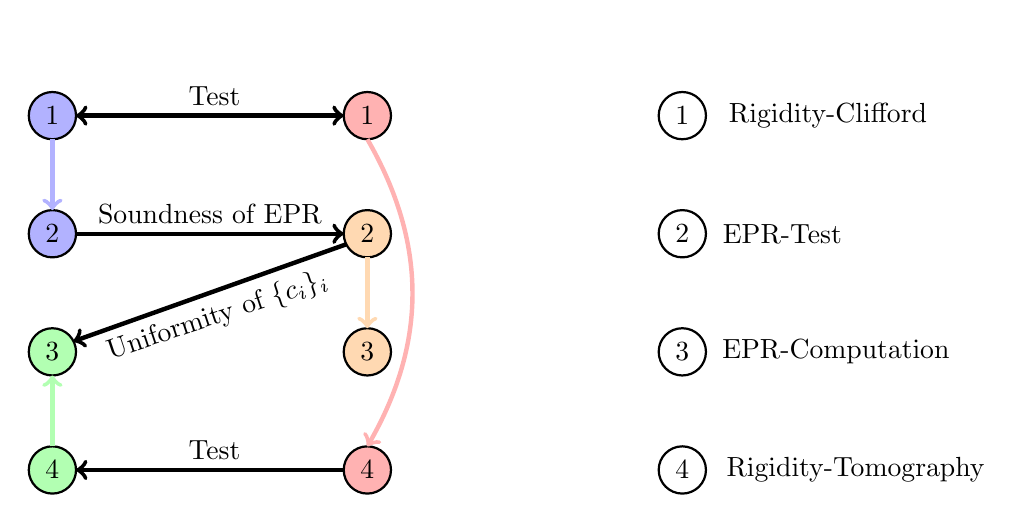
\begin{tikzpicture}
\filldraw[thick, fill=blue!30!white] (0,6) circle (.3);
\filldraw[thick, fill=blue!30!white] (0,4.5) circle (.3);
\filldraw[thick, fill=green!30!white] (0,3) circle (.3);
\filldraw[thick, fill=green!30!white] (0,1.5) circle (.3);

\filldraw[thick, fill=red!30!white] (4,6) circle (.3);
\filldraw[thick, fill=orange!30!white] (4,4.5) circle (.3);
\filldraw[thick, fill=orange!30!white] (4,3) circle (.3);
\filldraw[thick, fill=red!30!white] (4,1.5) circle (.3);

\node at (0,6) {1};
\node at (4,6) {1};
\node at (0,4.5) {2};
\node at (4,4.5) {2};
\node at (0,3) {3};
\node at (4,3) {3};
\node at (0,1.5) {4};
\node at (4,1.5) {4};

\draw[ultra thick, ->, blue!30!white] (0,5.7)--(0,4.8);
\draw[ultra thick, ->, green!30!white] (0,1.8)--(0,2.7);
\path[ultra thick, ->, orange!30!white] (4,4.2) edge (4,3.3);
\path[ultra thick, ->, red!30!white] (4,5.7) edge[bend left] (4,1.8);

\draw[ultra thick, <->] (.3,6)--(3.7,6);
\draw[ultra thick, ->] (.3,4.5)--(3.7,4.5);
\draw[ultra thick, <-] (.268,3.134)--(3.732,4.366);
\draw[ultra thick, <-] (.3,1.5)--(3.7,1.5);

\node at (2,6.25) {$\rigid$ Test};
\node at (2,4.75) {Soundness of EPR};
\node [rotate=18.5] at (2.1,3.45) {Uniformity of $\{c_i\}_i$};
\node at (2,1.75) {$\tom$ Test};

\draw[thick] (8,6) circle (.3);
\node at (8,6) {1};
\node at (9.85,6) {Rigidity-Clifford};

\draw[thick] (8,4.5) circle (.3);
\node at (8,4.5) {2};
\node at (9.27,4.5) {EPR-Test};

\draw[thick] (8,3) circle (.3);
\node at (8,3) {3};
\node at (9.95,3) {EPR-Computation};

\draw[thick] (8,1.5) circle (.3);
\node at (8,1.5) {4};
\node at (10.2,1.5) {Rigidity-Tomography};

\node at (0,7) {\pv};
\node at (4,7) {\pp};

%\draw (1.8,5.9) rectangle (2.2,5.5);
%\node at (2,5.7) {\small i};

%\draw (-.5,5.05) rectangle (-.1,5.45);
%\node at (-.3,5.25) {\small ii};

%\draw (4.65,3.55) rectangle (5.05,3.95);
%\node at (4.85,3.75) {\small iii};

%\draw (1.8,4.0) rectangle (2.2,4.4);
%\node at (2,4.2) {\small iv};

%\draw (4.05,3.95) rectangle (4.45,3.55);
%\node at (4.25,3.75) {\small vii};

%\draw (1.2,3.95) rectangle (.8,3.55);
%\node at (1,3.75) {\small iv};

%\draw (1.8,1.05) rectangle (2.2,1.45);
%\node at (2,1.25) {\small v};

%\draw (-.5,2.0) rectangle (-.1,2.4);
%\node at (-.3,2.2) {\small vi};


\end{tikzpicture}
\caption{Overview of the soundness of the Dog-Walker Protocol}\label{fig:full-dog-walker}
\end{figure}




\noindent The structure of the proof is as follows (see also Figure~\ref{fig:full-dog-walker}):
\begin{enumerate}
\item[(i)] By the game $\rigid$, in the Rigidity-Clifford rounds, both $\pp$ and $\pv$ must be honest, or they would lose the game.
\item[(ii)] Since $\pv$ can't distinguish between Rigidity-Clifford and EPR-Test (both are Figure \ref{fig:dogwalker-protocol-PV} Item 1 from his perspective, and the input distributions, while not identical, are within constant total variation distance), $\pv$ must be honest in the EPR-Test rounds, by (i). 
\item[(iii)] Since $\pp$ can't distinguish between Rigidity-Clifford and Rigidity-Tomography (both are Figure~\ref{fig:dogwalker-protocol-PP} Item 1 from his perspective), $\pp$ must be honest in the Rigidity-Tomography rounds, by~(i). 
\item[(iv)] Since $\pv$ is honest in EPR-Test rounds by (ii), $\pp$ must be honest in EPR-Test rounds or he will get caught, but in particular, he must output values $\{c_i\}_{i\in [t]}$ that are uniform random and independent of $\vec{z}$. Since $\pp$ can't distinguish between EPR-Test and EPR-Computation rounds, this is also true in EPR-Computation rounds, when the verifier sends the values $\{c_i\}_i$ to $\pv$. 
\item[(v)] $\pv$ must be honest in Rigidity-Tomography rounds, or the provers would lose the game $\tom$.
\item[(vi)] Since $\pv$ can't distinguish between Rigidity-Tomography rounds and EPR-Computation rounds (both are Figure \ref{fig:dogwalker-protocol-PV} Item 2 from his perspective), $\pv$ must be honest in EPR-Computation rounds, by~(v), and his input distribution to both rounds is within constant total variation distance, by (iv).
\item[(vii)] Since $\pv$ is honest in EPR-Test rounds by (ii), and EPR-Computation rounds by (vi), the combined behavior of $\ver$ and $\pv$ in the EPR rounds is that of $V_{EPR}$ in the EPR Protocol, so
by the soundness of the EPR Protocol, $\pp$ must be honest in EPR-Computation rounds, or get caught in the EPR-Test rounds with high probability.
\end{enumerate}

 The following lemma establishes (i), (ii) and (iii). 

\begin{lemma}\label{lem:PV-2-PP-4}
Suppose the verifier executes the Dog-Walker Protocol 
with provers $(\pv^*,\pp^*)$ such that the provers are accepted with probability $q_1\geq 1-\eps$ in the Rigidity-Clifford Round, $q_2$ in the EPR-Test Round, $q_3$ in the EPR-Computation Round, and $q_4$ in the Rigidity-Tomography Round. Then there exist provers $(\pv',\pp')$ such that:
\begin{itemize}[nolistsep]
\item $\pv'$ and $\pp'$ both apply the honest strategy in the Rigidity-Clifford rounds, $\pv'$ applies the honest strategy in the EPR-Test rounds, and $\pp'$ applies the honest strategy in the Rigidity-Tomography rounds; in particular, the state shared by the provers at the beginning of the protocol is a tensor product of the honest state consisting of $m$ shared EPR pairs and an arbitrary shared ancilla;
\item The provers are accepted with probability $q_2'=q_2-O(\mathrm{poly}(\eps))$ in the EPR-Test Round, $q_3'=q_3$ in the EPR-Computation Round, and $q_4'=q_4-O(\mathrm{poly}(\eps))$ in the Rigidity-Tomography Round. 
\end{itemize}
\end{lemma}

\begin{proof}
Using a similar argument as in Lemma~\ref{soundlemma}, the strategy of $\pv^*$ in
Rigidity-Clifford rounds, which is also his strategy in EPR-Test rounds (Figure \ref{fig:dogwalker-protocol-PV} Item 1); and the strategy of $\pp^*$ in Rigidity-Clifford rounds, which is also his strategy in Rigidity-Tomography rounds (Figure \ref{fig:dogwalker-protocol-PP} Item 1);
 can both be replaced with the honest strategies. Since the distribution of inputs to $\pp^*$ in the Rigidity-Tomography rounds and Rigidity-Clifford rounds is the same, the success probability in the Rigidity-Tomography rounds is changed by at most $O(\mathrm{poly}(\eps))$ by using the honest strategy. 
On the other hand, $\pv^*$'s input distribution in EPR-Test rounds is uniform on $\Sigma^m$, whereas his distribution in Rigidity-Clifford rounds is given by $\mu$. However, from the description of the test $\rigid$ it is clear that for all $W\in\Sigma^m$, $\mu(W)\geq \frac{1}{c|\Sigma|^m}$ for some constant $c>1$, thus the total variation distance between the two distributions is at most $1-\frac{1}{c}$. Thus, replacing $\pv^*$ with the honest strategy in the EPR-Test  rounds will change the success probability by at most  $O(\mathrm{poly}(\eps))$. 

Finally, since the provers' strategy in the EPR-Computation round has not changed, the
  acceptance probability in it remains unchanged.
\end{proof}

Next, we will show that whenever $\pv^*$ is honest in the EPR-Test rounds this forces $\pp^*$ to output (close to) uniformly random $\{c_i\}_{i\in [t]}$ that are independent of the round type, even given $\vec{z}$. This will allow us to verify that $\pp^*$ is unable to signal to $\pv^*$ whether the round is an EPR Round in the EPR-Computation round, when $\pv^*$ is sent $\vec{z}$ and $\vec{c}$. This establishes (iv). 


\begin{lemma}\label{lem:ci-unif}
Suppose the verifier executes the Dog-Walker Protocol with provers $(\pv^*,\pp^*)$ such that the initial shared state of the provers consists of $m$ shared EPR pairs, together with an arbitrary shared auxiliary state; $\pv^*$ plays the honest strategy in the EPR-Test rounds; the provers are accepted with probability $q_1$ in the Rigidity-Clifford Round, $q_2 = 1-\eps'$ in the EPR-Test Round, $q_3$ in the EPR-Computation Round, and $q_4$ in the Rigidity-Tomography Round. Then the input $(\vec{c},\vec{z})$ given by the verifier to $\pv^*$ in the EPR-Computation rounds has a distribution that is within $O(\eps')$ total variation distance of uniform on $\{0,1\}^t\times\{0,1\}^t$. 
\end{lemma}

\begin{proof}
Let $a_i'$ denote the $\sf X$ key of the wire to which the $i$-th $\sf T$ gate is applied, just before the $i$-th $\sf T$ gate is applied, and let $D_i$ be a random variable defined as follows. If the $i$-th $\sf T$ gate is even, let $D_i=e_i+a_i'$, where we interpret $e_i$ and $a_i'$ as the random variables representing the measurement result and key $\ver$ would get if she chooses to execute an $X$-Test round. If the $i$-th $\sf T$ gate is odd, let $D_i=e_i+a_i'$, where we interpret $e_i$ and $a_i'$ as the measurement result and key $\ver$ would get if she chooses to execute an $Z$-Test round. Since $\pv^*$ is assumed to play honestly in EPR-Test rounds, $\vec{D}$ is uniformly distributed in $\{0,1\}^t$. In particular, we have, for any $\vec{d},\vec{z}\in\{0,1\}^t$,
\begin{equation}
\Pr[\vec{D}=\vec{d},\vec{Z}=\vec{z}]=\frac{1}{4^t}.\label{eq:D-unif}
\end{equation}

Let $C_i$ be the random variable that corresponds to the measurement output of
  the $i$-th $\sf T$ gadget by $\pp^*$ in $X$-Test round if the $i$-th $\sf T$
  gate is even, or the measurement output of the $i$-th $\sf T$ gadget 
  by $\pp^*$ in $Z$-Test round if the $i$-th $\sf T$ gate is odd.

Let $T^0\subset[t]$ be the set of even $\sf T$ gates and $T^1\subset[t]$ the set of odd $\sf T$ gates. In an $X$-Test Round, the provers are rejected whenever $i\in T^0$ and $c_i\neq d_i$, and in a $Z$-Test Round, they are rejected whenever $i\in T^1$ and $c_i\neq d_i$. An EPR-Test Round consists of running one of these two rounds with equal probability, so:
\begin{equation}
\Pr[\vec{C}\neq\vec{D}]  \leq  2\eps'.\label{eq:C-D-equal}
\end{equation}
We can express \eqref{eq:C-D-equal} as
\begin{equation*}
\Pr[(\vec{C},\vec{Z})\neq(\vec{D},\vec{Z})]  \leq  2\eps'.
\end{equation*}
We conclude by using the easily verifiable fact that for any random variables $X$ and $Y$ such that $\Pr[X= Y]\geq 1-2\eps'$, the total variation distance between the marginal distributions on $X$ and $Y$ is at most $2\eps'$. 
\end{proof}

Next, we can use the tomography test $\tom$ to establish (v), and then the fact that by Lemma \ref{lem:ci-unif} the input to $\pv$ is not very different in EPR-Computation and Rigidity-Tomography rounds to establish (vi):

\begin{lemma}\label{lem:PV-34}
Suppose the verifier executes the Dog-Walker Protocol with provers $(\pv^*,\pp^*)$ such that: $\pv^*$ applies the honest strategy in EPR-Test rounds; 
$\pp^*$ applies the honest strategy in the Rigidity-Tomography rounds; and the provers are accepted with probability $q_1$ in the Rigidity-Clifford Round, $q_2 = 1-\eps'$ in the EPR-Test Round, $q_3$ in the EPR-Computation Round, and $q_4=1-\eps$ in the Rigidity-Tomography Round. Then there exist provers $(\pv',\pp')$ such that $\pv'$ applies the honest strategy in the Rigidity-Tomography rounds and EPR-Computation rounds, $\pp'$ applies the honest strategy in Rigidity-Tomography rounds, and
the provers are accepted with probability $q_1$ in the Rigidity-Clifford Round, $q_2 = 1-\eps'$ in the EPR-Test Round and $q_3-\mathrm{poly}(\eps)-O(\eps')$ in the EPR-Computation round. 
\end{lemma}

\begin{proof}
The Rigidity-Tomography rounds can be seen as $\ver$ playing the Tomography Game
  with the provers, except that whereas $\pv^*$ gets no non-trivial input in the
  Tomography Game, in the Rigidity-Tomography round, he gets random values
  $\vec{c}$ and $\vec{z}$ on which his strategy can depend. Fix $\vec{x}$, and let
  $\{Q_{\vec{c},\vec{z}}^{u}\}_{u}$ be the projective measurement that $\pv^*$
  applies upon receiving $\vec{c},\vec{z},\vec{x}$, where  $u = (\vec{d},\vec{e})$ is
  the string of outcomes obtained by $\pv$ on the $n+t$ single-qubit
  measurements he is to perform according to Step 2 in
  Figure~\ref{fig:dogwalker-protocol-PV}. 

By Corollary \ref{cor:clifford-rigid-adaptive}, since the provers win the Rigidity-Tomography round with probability $1-\eps$, for every $\vec{c},\vec{z}\in\{0,1\}^t$,
there exist distributions $q_{\vec{c},\vec{z}}$ on $\Sigma^m\times\{\pm\}$ such that the following is $O(\mathrm{poly}(\eps))$:
\begin{equation}\label{eq:big-dist}
\Es{\vec{c},\vec{z}}\sum_{ u\in \{0, 1\}^m}
\Big\| \Tr_{\reg{A},\hat{\reg{B}}}\left((\Id_{\reg{A}}\otimes V_{\reg{B}} Q_{\vec{c},\vec{z}}^{u})\ket{\psi}\bra{\psi}_{\reg{AB}}(\Id_{\reg{A}}\otimes V_{\reg{B}} Q_{\vec{c},\vec{z}}^{u})^\dagger\right)
- \sum_{\lambda\in\{\pm\}}q_{\vec{c},\vec{z}}(W',\lambda)\left(\bigotimes_{i=1}^m \frac{\sigma^{u_i}_{W_i',\lambda}}{2}\right)\Big\|_1. 
\end{equation}
Here we use the notation from Corollary \ref{cor:clifford-rigid} and
  \ref{cor:clifford-rigid-adaptive}. The string
  $W'=W(\vec{c},\vec{z},\vec{u})\in\Sigma^m$ is uniquely determined by
  $\vec{c},\vec{z}$, and the outcomes ${u}$ reported by $\pv^*$; indeed it
  is using this string that $\pv^*$'s answers are checked against the
  measurement outcomes obtained by $\pp^*$, who by assumption applies the
  honest strategy. For any fixed $(W',\lambda)$ the distribution on
  outcomes $u$ obtained in the ``honest'' strategy represented by the right-hand
  side in~\eqref{eq:big-dist} is uniform. Thus the outcomes $u$ reported by
  $\pv^*$ are within $\poly(\eps)$ of uniform. From this it follows that the joint distribution on transcripts $(\vec{c},\vec{z},u,W'=W(\vec{c},\vec{z},u))$ that results from an interaction with $\pv^*$ is within statistical distance $\poly(\eps)$ of the distribution generated by an interaction with the honest $\pv$; furthermore, by~\eqref{eq:big-dist} the resulting post-measurement states on $\pp^*$ are also $\poly(\eps)$ close to the honest ones, on average over this distribution. 

We can now consider two provers $\pv'$ and $\pp'$ who, in Rigidity-Tomography rounds, first apply the isometries $V_A$, $V_B$ from Corollary~\ref{cor:clifford-rigid-adaptive}, then  measure their auxiliary systems $\hat{\reg{A}}$ and $\hat{\reg{B}}$ using $\Delta_Y$, obtaining a shared outcome $\lambda\in\{\pm\}$, and finally apply the honest strategy shown in Item 2 of Figure \ref{fig:dogwalker-protocol-PV} ($\lambda=+$) or its conjugate ($\lambda = -$). Furthermore, conjugating the honest strategy produces exactly the same statistics as the honest strategy itself, so we may in fact assume that $\pv'$ and $\pp'$ both apply the honest strategy in Rigidity-Tomography rounds. 


A consequence of $\pv'$ applying the honest strategy in Figure \ref{fig:dogwalker-protocol-PV} Item 2 is that $\pv'$ also plays the honest strategy in EPR-Computation rounds. Since $\pv'$ is still honest in the EPR-Test round and $q_2 = 1-\eps'$, Lemma \ref{lem:ci-unif} implies that the distribution of the input to $\pv'$ in EPR-Computation rounds is within $\poly(\eps)+O(\eps')$ total variation distance of his input in
Rigidity-Tomography rounds, therefore the provers' success probability in EPR-Computation rounds changes at most by $\mathrm{poly}(\eps)+O(\eps')$. 
\end{proof}


Finally, we show that if $\pv$ is honest, $\pp$ must be honest in EPR computation rounds, or the acceptance probability would be low, establishing (vii):
\begin{lemma}\label{lem:PP-3}
Suppose $\ver$ %the verifier
 executes the Dog-Walker Protocol on an input $(Q,\ket{\vec{x}})$ such that $\norm{\Pi_0 Q\ket{\vec{x}}}^2\leq 1/3$, with provers $(\pv,\pp)$ such that $\pv$ plays the honest strategy. Let $q_2$ be the provers' acceptance probability in EPR-Test rounds. Then the verifier accepts with probability at most
  $p_1(1-\delta_c) +p_2q_2+p_3(5/3-4q_2/3)+p_4$. 
\end{lemma}
\begin{proof}
With probability $p_2+p_3$, $\ver$ executes an EPR round, in which case, she executes EPR-Computation with probability $\frac{p_3}{p_2+p_3}$ and EPR-Test with probability $\frac{p_2}{p_2+p_3}$. In the former case, since $\pv$ is honest, he is executing $V_{EPR}^0$. In fact, the behavior of an honest $\pv$ in the EPR-Test rounds is also that of $V_{EPR}^r$. Thus, the combined behavior of $\ver$ and $\pv$ is that of $V_{EPR}$. Then the result follows from Theorem \ref{thm:EPR-soundness}. 
\end{proof}

We can now combine Lemmas \ref{lem:PV-2-PP-4}, \ref{lem:PV-34}, and \ref{lem:PP-3} to get the main result of this section, the ``soundness'' part of Theorem~\ref{thm:dog-walker}.

\begin{lemma}[Constant soundness-completeness gap]\label{lem:dogwalker-soundness}
 There exist constants $p_1$, $p_2$, $p_3$, $p_4=1-p_1-p_2-p_3$ and $\Delta>0$ such that if the verifier executes the Dog-Walker Protocol with parameters $(p_1,p_2,p_3,p_4)$ on input $(Q,\ket{\vec{x}})$ such that $\norm{\Pi_0 Q\ket{\vec{x}}}^2\leq 1/3$, then any provers $(\pv^*,\pp^*)$ are accepted with probability at most $p_{\mathrm{sound}}=p_{\mathrm{compl}}-\Delta$. 
\end{lemma}

\begin{proof}
Suppose the provers $\pv^*$ and $\pp^*$ are such that the lowest acceptance probability in either the Rigidity-Clifford round or the Rigidity-Tomography round is $1- \eps$, and they are accepted with probability $1-\eps'$ in the EPR-Test round, and with probability $1/3+w$ in the Computation Round. Applying  Lemma \ref{lem:PV-2-PP-4} and Lemma \ref{lem:PV-34} in sequence, we deduce the existence of provers $(\pv',\pp')$ for which
\begin{align*}
q_1' &= 1- O(\delta_c), \\  q_2' &= 1-\eps'- \poly(\eps), \\ q_3' &= \frac13+w-
  \poly(\eps)-O(\eps'),\\ q_4' &= 1,
\end{align*}
where $q'_1$, $q'_2$, $q'_3$ and $q'_4$ are their success probabilities in the
  four types of rounds, and $1-\delta_c$ is the completeness of the
  $\rigid$ test; from Corollary~\ref{cor:clifford-rigid} we have $\delta_c = 2^{-\Omega(n+t)}$. Moreover $\pv'$ applies the honest strategy in all rounds, while $\pp'$ applies the honest strategy in the Rigidity-Clifford and Rigidity-Tomography rounds. Applying Lemma \ref{lem:PP-3}, it follows that 
$$w \,\leq\, O(\eps') + \poly(\eps) +p_1 \cdot O(\delta_c).$$
Therefore the prover's overall success probability is at most 
\begin{align*}
& \min(p_1,p_4)(1-\eps)+\max(p_1,p_4) + p_2(1-\eps')+p_3\left(\frac{1}{3}+w\right) \\
\leq & p_{\mathrm{compl}} - \left( \frac{p_3}{3} + \eps' p_2+\eps\min(p_1,p_4)\right)+ p_3\left(O(\eps')+\poly(\eps)\right)+ (p_1 + p_3p_1) \cdot O(\delta_c),
\end{align*}
where recall from Lemma~\ref{lem:dogwalker-completeness} that
  $p_{\mathrm{compl}} =  p_1(1-\delta_c)+p_2+p_4+\frac{2}{3}p_3$. Fixing $p_2$
  to be a large enough multiple of $p_1$ and of $p_3$ we can ensure that the net contribution
  of the terms involving $\eps'$ and $\delta_c$ on the right-hand side is always
  non-positive. Choosing $p_1=p_4$ and $p_3$ so that the ratio $p_3/p_1$ is small
  enough we can ensure that the right-hand side is less than $p_{\mathrm{compl}}
  -\Delta$, for some universal constant $\Delta>0$ and all $\eps,\eps'\geq 0$.
\end{proof}



\subsection{Two-prover game for QMA}\label{sec:qma}

In this section we propose a new two-prover game for QMA, which is based on the Dog-Walker
protocol. Such type of games are important in the context of the Quantum PCP conjecture~\cite{AharonovAV13}, more specifically to its game version that was recently proved~\cite{NatarajanV18}.


A promise problem $L$ is in QMA if there is a uniform family
of quantum circuits $\{V_x\}_{x \in L}$ such that if $x$ is a yes-instance, then there exists a
quantum state $\ket{\psi} \in \left(\C^2\right)^{\otimes n_w}$, such that
$V_x$  accepts on input $\ket{\psi}\ket{0}^{\otimes n_a}$ with probability at least
$\frac{2}{3}$, while for a no-instance $x$ and  all states $\ket{\psi} \in
\left(\C^2\right)^{\otimes n_w}$, $V_x$
rejects on input $\ket{\psi}\ket{0}^{\otimes n_a}$ with probability at
least $\frac{2}{3}$. The run-time of the circuit $V_x$ and the values $n_w$ and $n_a$ are polynomially bounded in $|x|$.

 In a multi-prover game for a promise problem $L$, an
 instance $x \in L$ is reduced to a game $G_x$ such that if $x$ is a yes-instance, then the maximum
 acceptance probability in the game is at least $c$, whereas if $x$ is a
 no-instance,
 then the maximum acceptance probability in the game is  at most $s$, for $c
 > s$.

 Here, we are interested in multi-prover games where the verifier is classical,
 the honest provers run a polynomially bounded quantum computation on copies
 of an accepting witness and the completeness-soundness gap $c-s$ is constant.
Using the Dog-Walker protocol, we are able to construct, to the best of our knowledge, the first two-prover
game for QMA with these parameters. In our protocol the Verifier and provers exchange messages of polynomial size 
in two rounds of communication, one with each
prover.

Our protocol consists in the Verifier running the Dog-Walker protocol,
  with the following changes:
  \begin{itemize}
    \item On X-Test rounds (resp.\ $Z$ Test-rounds), the Verifier randomly selects  positions where
      $\pv$ has measured in the $Z$ basis (resp.\ $X$ basis) and sends them to $\pp$. $\pp$ uses the EPR pair halves in these positions as the witness register when he executes the circuit $V_x$.
    \item On Rigidity-Computation rounds, the Verifier
      informs $\pv$ of the halves of EPR pairs that should be used to teleport the witness
      state to $\pp$, and $\pv$ reports the outcomes of the teleportation
      measurements along with the answers for the original Dog-Walker protocol. The Verifier ignores the measurements corresponding to the teleportation and uses the remaining bits to perform the same checks as in the original Dog-Walker protocol.
      \item On EPR-Computation rounds, the Verifier informs $\pp$ of the
      EPR pair halves that should be used as the witness when he performs the circuit $V_x$.  
      The Verifier
      also informs $\pv$ of these positions, who should use them to teleport the witness
      state to $\pp$.  The outcomes of the teleportation      measurements are reported to the Verifier along with the answers for the original Dog-Walker protocol, in order that the Verifier can decrypt the output of the computation.
  \end{itemize}

The full description of the protocol is presented in Figures~\ref{fig:qma-protocol-V}, \ref{fig:qma-protocol-PP} and \ref{fig:qma-protocol-PV}, where the differences to the original Dog-Walker protocol are underlined. We state the result and sketch its proof. 


%----------------%
\begin{figure}[H]
\rule[1ex]{\textwidth}{0.5pt}
\vspace{-20pt}
\justify
Let $x$ be an instance of a language $L \in$ QMA and $V_x$ the associated verification circuit. $V_x$ takes as input  an $n_w$-qubit witness register and an $n_a$-qubit ancilla register. It has $t$ $\sf T$ gates, $t_0$ of which are even and $t-t_0$ are odd (see Section~\ref{sec:EPR-protocol} for the definition of even and odd $\sf T$ gates).

\justify
1. Select a round type \textbf{EPR} or \textbf{Rigidity}, and disjoint sets
  $N^w,N^a, T^0,T^1\subset \{1,\ldots,m\}$ of sizes $n_w$, $n_a$,  $t_0$ and $t-t_0$ respectively. 
\begin{description}
\item[EPR] Choose $\vec{z}$ uniformly at random from $\{0,1\}^t$ and send it,
  along with $\vec{x}$, $N^w$, $N^a$, $T^0$ and $T^1$, to $\pp$. Receive measurement outcomes $\vec{c}\in\{0,1\}^t$ and $c_f\in\{0,1\}$ from $\pp$.
\item[Rigidity] Choose $W'$ according to $\mu(\cdot)$ and send it to $\pp$. Receive $\vec{e}'\in \{0,1\}^m$ from $\pp$. 
\end{description}
2. Select a sub-round type at random from \textbf{Computation}, \textbf{X-Test} or \textbf{Z-Test}. 
\begin{description}
\item[Computation] Based on whether it's an \text{EPR} or a \text{Rigidity} Round:
	\begin{description}
	\item[EPR]
		\begin{enumerate}
		\item[(i)] Send $\vec{x}$, $\vec{z}$, $\vec{c}$ and sets \highlight{$N^w$}, $N^a$, $T^0$
      and $T^1$ to $\pv$, and receive measurement outcomes \highlight{$\vec{a},\vec{b}\in
        \{0,1\}^{n_w + n_a}$} and $\vec{e}\in\{0,1\}^t$.
		\item[(ii)] Apply the update rules from Table \ref{tab:EPR-key-updates} gate-by-gate to obtain the final $\sf X$ key for the output wire $a_f'$. If $c_f+a_f'\neq 0$, $\sf reject$. 
		\end{enumerate}
	\item[Rigidity (Tomography)]
		\begin{enumerate}
		\item[(i)] Choose uniform random strings $\vec{c},\vec{z}\in\{0,1\}^t$, $\vec{x} \in \{0,1\}^n$ 
      to send to $\pv$, along with \highlight{$N^w$}, $N^a$ and $T$, and receive measurement outcomes \highlight{$\vec{a}, \vec{b}\in \{0,1\}^{n_w + n_a}$} and $\vec{e}\in\{0,1\}^t$. 
		\item[(ii)]
		From $\vec{x}$, $\vec{c}$, $\vec{z}$, $\vec{a}$, $\vec{b}$ and $\vec{e}$, determine the adaptive measurements $W\in\Sigma^{n+t}$ that $V_{EPR}^0$ would have performed (based on Figure \ref{fig:original-protocol-VEPRr}), and $\sf reject$ if the input-output pairs $(W',\vec{e}')$ and $(N\cup T,(W,\vec{e}))$ do not satisfy the winning criterion for $\tom(\Sigma,n+t,m)$.
		\end{enumerate}
	\end{description}
\item[$X$-Test] Based on whether it's an \text{EPR} or a \text{Rigidity} Round:
\begin{description}
	\item[EPR] 
	\begin{enumerate}
		\item[(i)] Choose $W\in\Sigma^m$ uniformly at random among all strings
      satisfying: $W_i=Z$ for all $i\in \highlight{N^w} \cup N^a$; $W_i=Z$ for all $i\in T^0$; and $W_i\in\{X,Y\}$ for all $i\in T^1$. Send $W$ to $\pv$ and receive measurement results $\vec{e}\in\{0,1\}^m$. Let $(\vec{a},\vec{b})=(\vec{e}_N,0^n)$. 
		\item[(ii)] Apply update rules from Table \ref{tab:EPR-key-updates} gate-by-gate to obtain $\forall i\in [t]$ the $\sf X$ key before the $i$-th $\sf T$ gate is applied, $a_i'$, and the final $\sf X$ key for the output wire, $a_f'$. 
If $\exists i$ s.t.\ the $i$-th $\sf T$ gate is even and $c_i\neq a_i'+e_i$, $\sf reject$. If $c_f+a_f'\neq 0$, $\sf reject$. 
	\end{enumerate}
	\item[Rigidity (Clifford)] Choose ${W}$ according to the marginal conditioned on ${W}'$, $\mu(\cdot|{W}')$. 
	Send ${W}$ to $\pv$ and receive $\vec{e}\in\{0,1\}^m$. Reject if   $({W}',\vec{e}',{W},\vec{e})$ doesn't win $\rigid(\Sigma,m)$. 
\end{description}

\item[$Z$-Test] Based on whether it's an \text{EPR} or a \text{Rigidity} Round:
\begin{description}
	\item[EPR] 
	\begin{enumerate}
		\item[(i)] Choose $W\in\Sigma^m$ uniformly at random among all strings
      satisfying: $W_i=X$ for all $i\in \highlight{N^w} \cup N^a$; $W_i\in\{X,Y\}$ for all $i\in T^0$; and $W_i=Z$ for all $i\in T^1$. Send $W$ to $\pv$ and receive measurement results $\vec{e}\in\{0,1\}^m$. Let $(\vec{a},\vec{b})=(0^n,\vec{e}_N)$.
		\item[(ii)] Apply update rules from Table \ref{tab:EPR-key-updates} gate-by-gate to obtain $\forall i\in [t]$, the $\sf X$ key before the $i$-th $\sf T$ gate is applied, $a_i'$. 
If $\exists i$ s.t.\ the $i$-th $\sf T$ gate is odd and $c_i\neq a_i'+e_i$, $\sf reject$. 
	\end{enumerate}
	\item[Rigidity (Clifford)] Identical to $X$-Test case.
\end{description}
\end{description}
\rule[2ex]{\textwidth}{0.5pt}\vspace{-.5cm}
\caption{QMA Protocol: Verifier's point of view.}\label{fig:qma-protocol-V}
\end{figure}


\begin{figure}[H]
\rule[1ex]{\textwidth}{0.5pt}
\vspace{-20pt}
\begin{enumerate}
  \item If $\pp$ receives a question ${W}'$ from $\ver$ (he is playing $\tom$ or $\rigid$):
\begin{enumerate}
     \item[]  Measure the $m$ qubits in the observable indicated by $W'$ --- for example, if $W'\in\Sigma^m$, for $i\in \{1,\ldots,m\}$, measure the $i$-th qubit in the basis indicated by $W_i'$ --- and report
       the outcomes $\vec{e}'$ to~$\ver$.
\end{enumerate}
\item If $\pp$ receives $\vec{x}, \vec{z}$, and sets $N^w$,$N^a$, $T^0$ and $T^1$ from $\ver$ (he is playing the role of $P_{EPR}$ from the EPR Protocol):
\begin{enumerate}
     \item[] Run  prover $P_{EPR}$ from Figure
       \ref{fig:original-protocol-PEPR} with the $V_x$ as the circuit $Q$, on input $\vec{z}$, \highlight{the $n_w$ qubits in $N^w$ as the witness}, the $n_a$ qubits in 
        $N^a$ as the ancilla, and the $t$ qubits in $T^0\cup T^1$ for $\sf T$ gadgets.
     Report the outputs $\vec{c}\in\{0,1\}^t$ and $c_f\in\{0,1\}$ of $P_{EPR}$  to $\ver$. 
\end{enumerate}
\end{enumerate}
\rule[2ex]{\textwidth}{0.5pt}\vspace{-.5cm}
\caption{QMA Protocol: Honest strategy for $\pp$.}\label{fig:qma-protocol-PP}
\end{figure}


\begin{figure}[H]
\rule[1ex]{\textwidth}{0.5pt}
\vspace{-20pt}
\begin{enumerate}
  \item If $\pv$ receives a question ${W}$ from $\ver$ (he is playing $\rigid$ or an $X$- or $Z$-Test Round):
\begin{enumerate}
     \item[]  Measure the $m$ qubits in the observable indicated by $W$ --- for example, if $W\in \Sigma^m$, for $i\in \{1,\ldots,m\}$, measure the $i$-th qubit in the basis indicated by $W_i$ --- and report the outcomes $\vec{e}$ to $\ver$.
\end{enumerate}

  \item If $\pv$ receives $\vec{x}$, $\vec{z}$, $\vec{c}$ and sets $N^w$, $N^a$, $T^0$ and $T^1$ from $\ver$ (he is playing $\tom$ or a Computation Round):
\begin{enumerate}
  \item[] \highlight{Using the EPR pairs in $N^w$, teleports the witness state
    $\ket{\psi}$ that makes $V_x$ accept with high probability. Let $(\vec{a}_{N^w}, \vec{b}_{N^w})$ be the corresponding
    outcomes of the teleportation measurements.}
  \item[] Measure each qubit in $N^a$ in the $Z$ basis with outcomes $\vec{d}$  and let $(\vec{a}_{N^a},
    \vec{b}_{N^a}) = (\vec{d}, \vec{0} )$ 
	\item[] Run the second step of procedure $V_{EPR}^0$ from Figure
    \ref{fig:original-protocol-VEPRr} with $V_x$ as the circuit $Q$, and the
    values $\vec{c}$, $\vec{z}$, \highlight{the $n_w$ qubits in $N^w$ as the witness}, the $n_a$ qubits in 
        $N^a$ as the ancilla, and the $t$ qubits in $T^0\cup T^1$ for $\sf T$ gadgets. Report the outputs  $\vec{a}$, $\vec{b}$ and $\vec{e}$ of $V_{EPR}^0$ to $\ver$.
\end{enumerate}
\end{enumerate}
\rule[2ex]{\textwidth}{0.5pt}\vspace{-.5cm}
\caption{QMA Protocol: Honest strategy for $\pv$.}\label{fig:qma-protocol-PV}
\end{figure}




\begin{lemma}
There
  exists universal constants $0\leq p_{compl}\leq 1$ and $\Delta >0$ such that the following holds. 
Let $L$ be a language in QMA and $x$ an instance of $L$ such that $n = |x|$. Let  $V_x$ be the
  verification circuit for this instance and $g$ the number of gates in $V_x$
  (in the compiled form as described in Section \ref{sec:prelim}). Then there exists a two-round interactive protocol
between a classical verifier and two entangled provers where the Verifier
sends  $O(n + g)$-bit questions to the provers, the provers answer with $O(n + g)$ bits and the protocol satisfies the following properties.
\begin{description}
\item[Completeness:] If $x$ is a yes-instance, then  there is a strategy for the provers such that the Verifier accepts with probability  at least $p_{compl}$.
\item[Soundness:] If $x$ is a no-instance, then for all strategies of the provers, the Verifier accepts with  probability at most
$p_{sound} = p_{compl} - \Delta$.
\end{description}
\end{lemma}
\begin{proof}[Proof sketch]
The Verifier performs the operations described in Figure~\ref{fig:qma-protocol-V}. 

  The completeness of the protocol is straightforward: if $\pp$ and $\pv$ use the strategy in Figures~\ref{fig:qma-protocol-PP} and \ref{fig:qma-protocol-PV}, respectively, then the Verifier accepts with  high probability.

  The soundness of the protocol follows from the combination of the soundness of the
  Dog-Walker protocol and the soundness of the QMA verification circuit. Along the same lines as 
  Lemmas~\ref{lem:PV-2-PP-4}, \ref{lem:ci-unif} and \ref{lem:PV-34},
  we can show that if
  the acceptance probability in Rigidity-Test, Rigidity-Computation and
  EPR-Test rounds
  is sufficiently high, then there is a strategy where the provers follow the honest
  strategy and the acceptance probability in EPR-Computation round is only slightly
  changed.  
  In the case where the provers are honest in the Rigidity-Test, Rigidity-Computation and EPR-Test rounds, no matter which state is held
  by $\pp$ as witness state, $V_x$ rejects with high probability in the EPR-Computation round, by the
  soundness of the QMA verification circuit.  The proof of soundness can be completed by repeating the
  arguments in Lemma~\ref{lem:dogwalker-soundness}.
\end{proof}



\subsection{Multi-prover game for QMA}\label{sec:qma}

In this section we propose a new multi-prover game for QMA, which is based on the Dog-Walker
protocol.
Recently, there has been an effort to devise such games~\cite{FitzsimonsV15,Ji16,natarajan2016robust},
due to their connections to the quantum PCP conjecture~\cite{AharonovAV13}.


A promise problem $L$ is in QMA if there is a uniform family
of quantum circuits $\{V_x\}_{x \in L}$ such that if $x$ is a yes-instance, then there exists a
quantum state $\ket{\psi} \in \left(\C^2\right)^{\otimes n_w}$, such that
$V_x$  accepts on input $\ket{\psi}\ket{0}^{\otimes n_a}$ with probability at least
$\frac{2}{3}$, while for a no-instance $x$ and  all states $\ket{\psi} \in
\left(\C^2\right)^{\otimes n_w}$, $V_x$
rejects on input $\ket{\psi}\ket{0}^{\otimes n_a}$ with probability at
least $\frac{2}{3}$. The run-time of the circuit $V_x$ and the values $n_w$ and $n_a$ are polynomially bounded in $|x|$.

 In a multi-prover game for a promise problem $L$, an
 instance $x \in L$ is reduced to ja game $G_x$ such that if $x$ is a yes-instance, then the maximum
 acceptance probability in the game is at least $c$, whereas if $x$ is a
 no-instance,
 then the maximum acceptance probability in the game is  at most $s$, for $c
 > s$.

 Here, we are interested in multi-prover games where the verifier is classical,
 the honest provers run a polynomially bounded quantum computation on copies
 of an accepting witness and the completeness-soundness gap $c-s$ is constant.
Using the Dog-Walker protocol, we are able to construct, to the best of our knowledge, the first two-prover
game for QMA with these parameters. In our protocol the Verifier and provers exchange messages of polynomial size 
in two rounds of communication, one with each
prover.

Our protocol consists in the Verifier running the Dog-Walker protocol,
  with the following changes:
  \begin{itemize}
    \item On X-Test rounds (resp.\ $Z$ Test-rounds), the Verifier randomly selects  positions where
      $\pv$ has measured in the $Z$ basis (resp.\ $X$ basis) and sends them to $\pp$. $\pp$ uses the EPR pair halves in these positions as the witness register when he executes the circuit $V_x$.
    \item On Rigidity-Computation rounds, the Verifier
      informs $\pv$ of the halves of EPR pairs that should be used to teleport the witness
      state to $\pp$, and $\pv$ reports the outcomes of the teleportation
      measurements along with the answers for the original Dog-Walker protocol. The Verifier ignores the measurements corresponding to the teleportation and uses the remaining bits to perform the same checks as in the original Dog-Walker protocol.
      \item On EPR-Computation rounds, the Verifier informs $\pp$ of the
      EPR pair halves that should be used as the witness when he performs the circuit $V_x$.  
      The Verifier
      also informs $\pv$ of these positions, who should use them to teleport the witness
      state to $\pp$.  The outcomes of the teleportation      measurements are reported to the Verifier along with the answers for the original Dog-Walker protocol, in order that the Verifier can decrypt the output of the computation.
  \end{itemize}

The full description of the protocol is presented in Figures~\ref{fig:qma-protocol-V}, \ref{fig:qma-protocol-PP} and \ref{fig:qma-protocol-PV}, where the differences to the original Dog-Walker protocol are underlined. We state the result and sketch its proof. 


%----------------%
\begin{figure}[H]
\rule[1ex]{\textwidth}{0.5pt}
\vspace{-20pt}
\justify
Let $x$ be an instance of a language $L \in$ QMA and $V_x$ the associated verification circuit. $V_x$ takes as input  an $n_w$-qubit witness register and an $n_a$-qubit ancilla register. It has $t$ $\sf T$ gates, $t_0$ of which are even and $t-t_0$ are odd (see Section~\ref{sec:EPR-protocol} for the definition of even and odd $\sf T$ gates).

\justify
1. Select a round type \textbf{EPR} or \textbf{Rigidity}, and disjoint sets
  $N^w,N^a, T^0,T^1\subset \{1,\ldots,m\}$ of sizes $n_w$, $n_a$,  $t_0$ and $t-t_0$ respectively. 
\begin{description}
\item[EPR] Choose $\vec{z}$ uniformly at random from $\{0,1\}^t$ and send it,
  along with $\vec{x}$, $N^w$, $N^a$, $T^0$ and $T^1$, to $\pp$. Receive measurement outcomes $\vec{c}\in\{0,1\}^t$ and $c_f\in\{0,1\}$ from $\pp$.
\item[Rigidity] Choose $W'$ according to $\mu(\cdot)$ and send it to $\pp$. Receive $\vec{e}'\in \{0,1\}^m$ from $\pp$. 
\end{description}
2. Select a sub-round type at random from \textbf{Computation}, \textbf{X-Test} or \textbf{Z-Test}. 
\begin{description}
\item[Computation] Based on whether it's an \text{EPR} or a \text{Rigidity} Round:
	\begin{description}
	\item[EPR]
		\begin{enumerate}
		\item[(i)] Send $\vec{x}$, $\vec{z}$, $\vec{c}$ and sets \highlight{$N^w$}, $N^a$, $T^0$
      and $T^1$ to $\pv$, and receive measurement outcomes $\vec{a},\vec{b}\in
        \{0,1\}^{n_w + n_a}$ and $\vec{e}\in\{0,1\}^t$.
		\item[(ii)] Apply the update rules from Table \ref{tab:EPR-key-updates} gate-by-gate to obtain the final $\sf X$ key for the output wire $a_f'$. If $c_f+a_f'\neq 0$, $\sf reject$. 
		\end{enumerate}
	\item[Rigidity (Tomography)]
		\begin{enumerate}
		\item[(i)] Choose uniform random strings $\vec{c},\vec{z}\in\{0,1\}^t$, $\vec{x} \in \{0,1\}^n$ 
      to send to $\pv$, along with \highlight{$N^w$}, $N^a$ and $T$, and receive measurement outcomes $\vec{a}, \vec{b}\in \{0,1\}^{n_w + n_a}$ and $\vec{e}\in\{0,1\}^t$. 
		\item[(ii)]
		From $\vec{x}$, $\vec{c}$, $\vec{z}$, $\vec{a}$, $\vec{b}$ and $\vec{e}$, determine the adaptive measurements $W\in\Sigma^{n+t}$ that $V_{EPR}^0$ would have performed (based on Figure \ref{fig:original-protocol-VEPRr}), and $\sf reject$ if the input-output pairs $(W',\vec{e}')$ and $(N\cup T,(W,\vec{e}))$ do not satisfy the winning criterion for $\tom(\Sigma,n+t,m)$.
		\end{enumerate}
	\end{description}
\item[$X$-Test] Based on whether it's an \text{EPR} or a \text{Rigidity} Round:
\begin{description}
	\item[EPR] 
	\begin{enumerate}
		\item[(i)] Choose $W\in\Sigma^m$ uniformly at random among all strings
      satisfying: $W_i=Z$ for all $i\in \highlight{N^w} \cup N^a$; $W_i=Z$ for all $i\in T^0$; and $W_i\in\{X,Y\}$ for all $i\in T^1$. Send $W$ to $\pv$ and receive measurement results $\vec{e}\in\{0,1\}^m$. Let $(\vec{a},\vec{b})=(\vec{e}_N,0^n)$. 
		\item[(ii)] Apply update rules from Table \ref{tab:EPR-key-updates} gate-by-gate to obtain $\forall i\in [t]$ the $\sf X$ key before the $i$-th $\sf T$ gate is applied, $a_i'$, and the final $\sf X$ key for the output wire, $a_f'$. 
If $\exists i$ s.t.\ the $i$-th $\sf T$ gate is even and $c_i\neq a_i'+e_i$, $\sf reject$. If $c_f+a_f'\neq 0$, $\sf reject$. 
	\end{enumerate}
	\item[Rigidity (Clifford)] Choose ${W}$ according to the marginal conditioned on ${W}'$, $\mu(\cdot|{W}')$. 
	Send ${W}$ to $\pv$ and receive $\vec{e}\in\{0,1\}^m$. Reject if   $({W}',\vec{e}',{W},\vec{e})$ doesn't win $\rigid(\Sigma,m)$. 
\end{description}

\item[$Z$-Test] Based on whether it's an \text{EPR} or a \text{Rigidity} Round:
\begin{description}
	\item[EPR] 
	\begin{enumerate}
		\item[(i)] Choose $W\in\Sigma^m$ uniformly at random among all strings
      satisfying: $W_i=X$ for all $i\in \highlight{N^w} \cup N^a$; $W_i\in\{X,Y\}$ for all $i\in T^0$; and $W_i=Z$ for all $i\in T^1$. Send $W$ to $\pv$ and receive measurement results $\vec{e}\in\{0,1\}^m$. Let $(\vec{a},\vec{b})=(0^n,\vec{e}_N)$.
		\item[(ii)] Apply update rules from Table \ref{tab:EPR-key-updates} gate-by-gate to obtain $\forall i\in [t]$, the $\sf X$ key before the $i$-th $\sf T$ gate is applied, $a_i'$. 
If $\exists i$ s.t.\ the $i$-th $\sf T$ gate is odd and $c_i\neq a_i'+e_i$, $\sf reject$. 
	\end{enumerate}
	\item[Rigidity (Clifford)] Identical to $X$-Test case.
\end{description}
\end{description}
\rule[2ex]{\textwidth}{0.5pt}\vspace{-.5cm}
\caption{QMA Protocol: Verifier's point of view.}\label{fig:qma-protocol-V}
\end{figure}


\begin{figure}[H]
\rule[1ex]{\textwidth}{0.5pt}
\vspace{-20pt}
\begin{enumerate}
  \item If $\pp$ receives a question ${W}'$ from $\ver$ (he is playing $\tom$ or $\rigid$):
\begin{enumerate}
     \item[]  Measure the $m$ qubits in the observable indicated by $W'$ --- for example, if $W'\in\Sigma^m$, for $i\in \{1,\ldots,m\}$, measure the $i$-th qubit in the basis indicated by $W_i'$ --- and report
       the outcomes $\vec{e}'$ to~$\ver$.
\end{enumerate}
\item If $\pp$ receives $\vec{x}, \vec{z}$, and sets $N^w$,$N^a$, $T^0$ and $T^1$ from $\ver$ (he is playing the role of $P_{EPR}$ from the EPR Protocol):
\begin{enumerate}
     \item[] Run  prover $P_{EPR}$ from Figure
       \ref{fig:original-protocol-PEPR} with the $V_x$ as the circuit $Q$, on input $\vec{z}$, \highlight{the $n_w$ qubits in $N^w$ as the witness}, the $n_a$ qubits in 
        $N^a$ as the ancilla, and the $t$ qubits in $T^0\cup T^1$ for $\sf T$ gadgets.
     Report the outputs $\vec{c}\in\{0,1\}^t$ and $c_f\in\{0,1\}$ of $P_{EPR}$  to $\ver$. 
\end{enumerate}
\end{enumerate}
\rule[2ex]{\textwidth}{0.5pt}\vspace{-.5cm}
\caption{QMA Protocol: Honest strategy for $\pp$.}\label{fig:qma-protocol-PP}
\end{figure}


\begin{figure}[H]
\rule[1ex]{\textwidth}{0.5pt}
\vspace{-20pt}
\begin{enumerate}
  \item If $\pv$ receives a question ${W}$ from $\ver$ (he is playing $\rigid$ or an $X$- or $Z$-Test Round):
\begin{enumerate}
     \item[]  Measure the $m$ qubits in the observable indicated by $W$ --- for example, if $W\in \Sigma^m$, for $i\in \{1,\ldots,m\}$, measure the $i$-th qubit in the basis indicated by $W_i$ --- and report the outcomes $\vec{e}$ to $\ver$.
\end{enumerate}

  \item If $\pv$ receives $\vec{x}$, $\vec{z}$, $\vec{c}$ and sets $N^w$, $N^a$, $T^0$ and $T^1$ from $\ver$ (he is playing $\tom$ or a Computation Round):
\begin{enumerate}
  \item[] \highlight{Using the EPR pairs in $N^w$, teleports the witness state
    $\ket{\psi}$ that makes $V_x$ accept with high probability. Let $(\vec{a}_{N^w}, \vec{b}_{N^w})$ be the corresponding
    outcomes of the teleportation measurements.}
  \item[] Measure each qubit in $N^a$ in the $Z$ basis with outcomes $\vec{d}$  and let $(\vec{a}_{N^a},
    \vec{b}_{N^a}) = (\vec{d}, \vec{0} )$ 
	\item[] Run the second step of procedure $V_{EPR}^0$ from Figure
    \ref{fig:original-protocol-VEPRr} with $V_x$ as the circuit $Q$, and the
    values $\vec{c}$, $\vec{z}$, \highlight{the $n_w$ qubits in $N^w$ as the witness}, the $n_a$ qubits in 
        $N^a$ as the ancilla, and the $t$ qubits in $T^0\cup T^1$ for $\sf T$ gadgets. Report the outputs  $\vec{a}$, $\vec{b}$ and $\vec{e}$ of $V_{EPR}^0$ to $\ver$.
\end{enumerate}
\end{enumerate}
\rule[2ex]{\textwidth}{0.5pt}\vspace{-.5cm}
\caption{QMA Protocol: Honest strategy for $\pv$.}\label{fig:qma-protocol-PV}
\end{figure}




\begin{lemma}
There
  exists universal constants $0\leq p_{compl}\leq 1$ and $\Delta >0$ such that the following holds. 
Let $L$ be a language in QMA and $x$ an instance of $L$ such that $n = |x|$. Let  $V_x$ be the
  verification circuit for this instance and $g$ the number of gates in $V_x$
  (in the compiled form as described in Section \ref{sec:prelim}). Then there exists a two-round interactive protocol
between a classical verifier and two entangled provers where the Verifier
sends  $O(n + g)$-bit questions to the provers, the provers answer with $O(n + g)$ bits and the protocol satisfies the following properties.
\begin{description}
\item[Completeness:] If $x$ is a yes-instance, then  there is a strategy for the provers such that the Verifier accepts with probability  at least $p_{compl}$.
\item[Soundness:] If $x$ is a no-instance, then for all strategies of the provers, the Verifier accepts with  probability at most
$p_{sound} = p_{compl} - \Delta$.
\end{description}
\end{lemma}
\begin{proof}[Proof sketch]
The Verifier performs the operations described in Figure~\ref{fig:qma-protocol-V}. 

  The completeness of the protocol is straightforward: if $\pp$ and $\pv$ use the strategy in Figures~\ref{fig:qma-protocol-PP} and \ref{fig:qma-protocol-PV}, respectively, then the Verifier accepts with  high probability.

  The soundness of the protocol follows from the combination of the soundness of the
  Dog-Walker protocol and the soundness of the QMA verification circuit. Along the same lines as 
  Lemmas~\ref{lem:PV-2-PP-4}, \ref{lem:ci-unif} and \ref{lem:PV-34},
  we can show that if
  the acceptance probability in Rigidity-Test, Rigidity-Computation and
  EPR-Test rounds
  is sufficiently high, then there is a strategy where the provers follow the honest
  strategy and the acceptance probability in EPR-Computation round is only slightly
  changed.  
  In the case where the provers are honest in the Rigidity-Test, Rigidity-Computation and EPR-Test rounds, no matter which state is held
  by $\pp$ as witness state, $V_x$ rejects with high probability in the EPR-Computation round, by the
  soundness of the QMA verification circuit.  The proof of soundness can be completed by repeating the
  arguments in Lemma~\ref{lem:dogwalker-soundness}.
\end{proof}



\section{Running our protocols in sequence}
\label{sec:sequential}


In this section, we describe a sequential procedure that, starting from our protocols in Sections \ref{sec:leash} and \ref{sec:dog-walker}, ensures that either the verifier aborts, or she obtains the correct outcome of the computation with probability $99\%$. Moreover, for honest provers, the probability that the procedure aborts is exponentially small in the number of sequential repetitions. Our sequential procedure has a number of rounds which depends on the desired soundness. As long as one only requires amplification of an arbitrarily small, but constant, soundness, to a fixed constant, the number of sequential repetitions remains constant.

To emphasize the importance of having such a sequential procedure, we note that, firstly, the current completeness-soundness gap between acceptance probability on \textit{yes} and \textit{no} instances, for both the leash and the Dog-Walker protocol, is a very small constant. Secondly, if a classical client wishes to employ our protocols to delegate a computation, we need to specify what the client interprets, at the end of the protocol, as the outcome of the delegated computation. The natural approach is to have the verifier interpret $\sf accept$ as a \textit{yes} outcome and $\sf reject$ as a \textit{no} outcome. However, this is not enough, as our security model based on the constant gap between acceptance probability for \textit{yes} and \textit{no} instances means that, while the provers have a low probability of making the verifier accept a \textit{no} instance as a $\textit{yes}$, they can always make the verifier accept a \textit{yes} instance as a \textit{no}, simply by behaving so that they are rejected.

The first point is addressed by running copies of the original protocol in sequence to amplify the completeness-soundness gap. The second point is addressed by having the verifier run the protocol twice: once for the circuit $Q$, and once for the circuit $Q'$ defined by appending an $\sf X$ gate to the output wire of $Q$. If $f:X\rightarrow \{0,1\}$ for some $X\subseteq \{0,1\}^n$ is defined by $f(x)=1$ if $\norm{\Pi_0 Q\ket{x}}^2\geq 2/3$, and $f(x)=0$ if $\norm{\Pi_0 Q\ket{x}}^2\leq 1/3$, i.e.\ $Q$ decides $f$ with bounded error $1/3$, then it is easy to see that $Q'$ decides $1-f$ with bounded error $1/3$. Thus, the verifier will accept $x$ as a \textit{yes} instance of $f$ if the protocol outputs ${\sf accept}$ when running $Q$ on $x$ and outputs $\sf reject$ when running $Q'$ on $x$. The verifier accepts $x$ as a \textit{no} instance of $f$ if the protocol outputs $\sf reject$ when running $Q$ on $x$ and outputs $\sf accept$ when running $Q'$ on $x$. The verifier aborts if she sees $\sf accept$-$\sf accept$ or $\sf reject$-$\sf reject$. 



\subsection{Sequential version of our protocols}

Let $P$ denote either the Verifier-on-a-leash or the Dog-Walker protocol from Sections \ref{sec:leash} and \ref{sec:dog-walker} respectively, and let $c$ and $\Delta$ denote the completeness and completeness-soundness gap. Let $\kappa$ be a security parameter.

\begin{figure}[H]
\rule[1ex]{\textwidth}{0.5pt}
\justify
Protocol $\mbox{Seq}(P,c,\Delta, \kappa)$: Let $(Q,x)$ be the verifier's input. 
\begin{enumerate}
\item The verifier runs $\kappa$ copies of protocol $P$ in sequence on input $(Q,x)$ with $\pp$ and $\pv$. Then she runs $\kappa$ copies in sequence on input $(Q',x)$. 
\item Let $\vec{o}, \vec{\tilde{o}} \in \{0,1\}^{\kappa}$ be such that $o_i = 1$ iff the $i$-th copy on input $(Q,x)$ accepts, and $\tilde{o}_i = 1$ iff the $i$-th copy on input $(Q',x)$ accepts. Let $wt(\vec{o})$ and $wt(\vec{\tilde{o}})$ be their Hamming weights. Then, the verifier accepts $1$ as the outcome of the delegated computation if $wt(\vec{o}) \geq (c- \frac{\Delta}{2}) \cdot \kappa$ and $wt(\vec{\tilde{o}}) < (c- \frac{\Delta}{2}) \cdot \kappa$, and she accepts $0$ as the outcome of the computation if $wt(\vec{o}) < (c- \frac{\Delta}{2})\cdot \kappa$ and $wt(\vec{\tilde{o}}) \geq (c- \frac{\Delta}{2}) \cdot \kappa$. Otherwise the verifier aborts.

\end{enumerate}
\rule[2ex]{\textwidth}{0.5pt}\vspace{-.5cm}
\caption{Sequential version of our protocols} \label{fig: gardenhose-protocol-parallel}
\end{figure}

\noindent We state and prove completeness and soundness for the sequential protocol.

\begin{theorem}
Let $c$ and $\Delta$ be respectively the completeness and completeness-soundness gap of protocol P. On input $(Q,x)$:
\begin{itemize}
\item If the provers are honest, $$ \Pr\big(\mbox{Seq}(P, c, \Delta, \kappa) \mbox{  outputs } f(x)\big) \geq 1 - 2\exp \left(-\frac{\Delta^2\kappa}{2}\right) .$$ 
\item For any cheating provers, $$\Pr\big(\mbox{Seq}(P, c, \Delta, \kappa) \mbox{  outputs } 1-f(x)\big) \leq \exp \left(-\frac{\Delta^2\kappa}{8}\right) .$$
\end{itemize}

\end{theorem}

\begin{proof} We first show completeness. 
Let $s = c- \Delta$ be the soundness of protocol P.
Suppose $f(x) = 1$ (the case $f(x) = 0$ is analogous). If the provers are honest, then the probability that the verifier outputs~$1$~is:
\begin{align*}
\Pr(\mbox{Verifier outputs $1$}) &= \Pr \left(wt(\vec{o}) \geq \left(c - \frac{\Delta}{2}\right)\cdot \kappa \,\, \land \,\, wt(\vec{\tilde{o}}) < \left(c - \frac{\Delta}{2}\right)\cdot \kappa \right)\\
&\geq 1-\Pr \left(wt(\vec{o}) < \left(c - \frac{\Delta}{2}\right)\cdot \kappa \right) - \Pr \left(wt(\vec{\tilde{o}}) \geq \left(c - \frac{\Delta}{2}\right)\cdot \kappa \right) \\
&\geq 1 - 2\exp \left(-\frac{\Delta^2\kappa}{2}\right)
\end{align*}
by Hoeffding's inequality.

Next we show soundness.
Again suppose $f(x) = 1$ (the case $f(x) = 0$ is analogous). Let $W_j$ be an indicator random variable for the event $\tilde{o}_j = 1$, and let $F_j = W_j - s$. Define $X_l = \sum_{j=1}^l F_j$, for $l=1,..,\kappa$. The $F_j$ define a submartingale with $|F_j| \leq 1 \,\, \forall j$. Hence, by Azuma's inequality, for any $\kappa\geq 1$, $\Pr(X_\kappa \geq t) \leq \exp(-\frac{t^2}{2\kappa})$. This implies that 
\begin{equation*}
\Pr \left(\sum_{j=1}^{\kappa} W_j - \kappa \cdot s \geq t \right) = \Pr \left(\sum_{j=1}^{\kappa}F_j \geq t \right) = \Pr \left(X_{\kappa} \geq t \right) \leq \exp\left(-\frac{t^2}{2\kappa}\, \right).
\end{equation*}
Then, for any provers $\pp$ and $\pv$,
\begin{align*}
\Pr(\mbox{Verifier outputs $0$}) &\leq \Pr \Big(wt(\vec{\tilde{o}}) \geq (c - \frac{\Delta}{2})\cdot \kappa \Big) \\
&= \Pr \left(\sum_{j=1}^\kappa W_j \geq (c - \frac{\Delta}{2})\cdot \kappa \right) \\
&= \Pr \left(\sum_{j=1}^{\kappa} W_j - \kappa \cdot s \geq \kappa \cdot \frac{\Delta}{2} \right) \\
&\leq \exp \left(-\frac{\Delta^2\kappa}{8}\right). 
\end{align*}
\end{proof}

